%%%%%%%%%%%%%%%%%%%%%%%%%%%%%%%%%%%%%%%%%%%%%%%%%%%%%%%%%%%%%%%%%%%%%%%
%%%%  Load the document class and packages                         %%%%
%%%%%%%%%%%%%%%%%%%%%%%%%%%%%%%%%%%%%%%%%%%%%%%%%%%%%%%%%%%%%%%%%%%%%%%
\documentclass[a4paper]{report}
\usepackage{epsfig}            % to insert PostScript figures
\graphicspath{ 
  {figs_compact2p/} 
}

%Change figure names
\renewcommand{\figurename}{Fig}

\usepackage[bf,footnotesize]{caption} % make captions small and label bold


\addtocounter{chapter}{1} %Because starting at zero is silly
\makeatletter
\renewcommand{\thesection}{\@arabic\c@section}
\renewcommand{\thefigure}{\@arabic\c@figure}
\makeatother

\usepackage[a4paper,margin=2.7cm,tmargin=2.5cm,bmargin=2.5cm]{geometry} 
\usepackage{textcomp}          % To make nice degree symbols and others\usepackage[bf,footnotesize]{caption} % make captions small and label bold
\usepackage{wrapfig}
%to produce the clickable references along the left in Acroread. This
%package must be included last. 
\usepackage[ps2pdf,bookmarks=TRUE]{hyperref} 



%%%%%%%%%%%%%%%%%%%%%%%%%%%%%%%%%%%%%%%%%%%%%%%%%%%%%%%%%%%%%%%%%%%%%%%
%%%%  Hypertext references for Acrobat                             %%%%
%%%%%%%%%%%%%%%%%%%%%%%%%%%%%%%%%%%%%%%%%%%%%%%%%%%%%%%%%%%%%%%%%%%%%%%
\hypersetup{
pdfauthor = {SWC},
pdftitle = {Custom Two Photon},
pdfkeywords = {optics, lenses, two photon, imaging, PMT, microscope},
pdfcreator = {LaTeX with hyperref},
pdfproducer = {dvips + ps2pdf}
           }


\begin{document}




%set the number of sectioning levels 
\setcounter{secnumdepth}{2}

\begin{center}
\textbf{\Large{Building a Custom Two Photon Microscope}}
\end{center}

\section{Introduction}
It is time to put together everything you've learned so far and build a two photon microscope. 
The microscope you will be building was designed specifically for this optics course and has the following features:

\begin{itemize}
\item A small footprint so two microscopes can be built simultaneously on a small optical table.
\item Modular design. e.g. the scanner relay optics can be assembled separately and just dropped into the microscope.
\item Light path remains low to the table for safety.
\item Low cost: almost all parts readily available from ThorLabs.
\end{itemize}


\section{IMPORTANT SAFETY INFORMATION}
Read this laser safety information before beginning. 
The following information should have been conveyed to you verbally. 
Please ask if you did not receive verbal instruction or if you have questions about laser safety. 

You will be working with a high energy pulsed laser capable of instantly blinding you should it enter your eye. 
During operation of the microscope the laser will be tuned to 920 nm which is invisible. 
Despite being invisible, the laser remains equally bright and equally dangerous.
Be very cautious around the set up:

\begin{itemize}
    \item Wear eye protection and use IR viewing cards as appropriate.
    \item Always be aware of the location of the beam and ensure everyone else in the room is also aware.
    \item Remove watches, jewelry, etc. Avoid directing the beam at shiny surfaces which could reflect it at unpredictable angles.
    \item Reduce laser power during alignment and tune the laser to visible wavelengths when possible.
    \item Shutter the beam when not using it. 
    \item Take particular care where the beam is directed upwards, such as in the periscope. 
    \item The scanners can deflect the beam by $>20$ degrees depending on the command signal. Ensure the mirrors are static and zeroed before routing the beam into the scan head for the first time. 
    \item Stand behind the scanners whilst the microscope is scanning.
    \item Use beam blocks where appropriate to keep the beam within your work area.
\end{itemize}

\clearpage

\section{General Plan}
Fig.~\ref{fig:layout} (left) shows the layout of key components on the optical table. 
The beam leaves the laser and enters a half-wave plate and polarizing beam-splitter cube that we will use to control laser power. 
The shutter is used to gate the beam for safety and not to fry the sample when you aren't scanning.
The beam proceeds to a beam expander and then on to the microscope. 
Fig.~\ref{fig:layout} (right) is a CAD model depicting the completed microscope. 
You will construct the beam expander and build the microscope. 
Since this involves a large number of parts, you will build it in stages as a series of modules then assemble those modules as a finished microscope. 
\begin{figure}[h]
\center
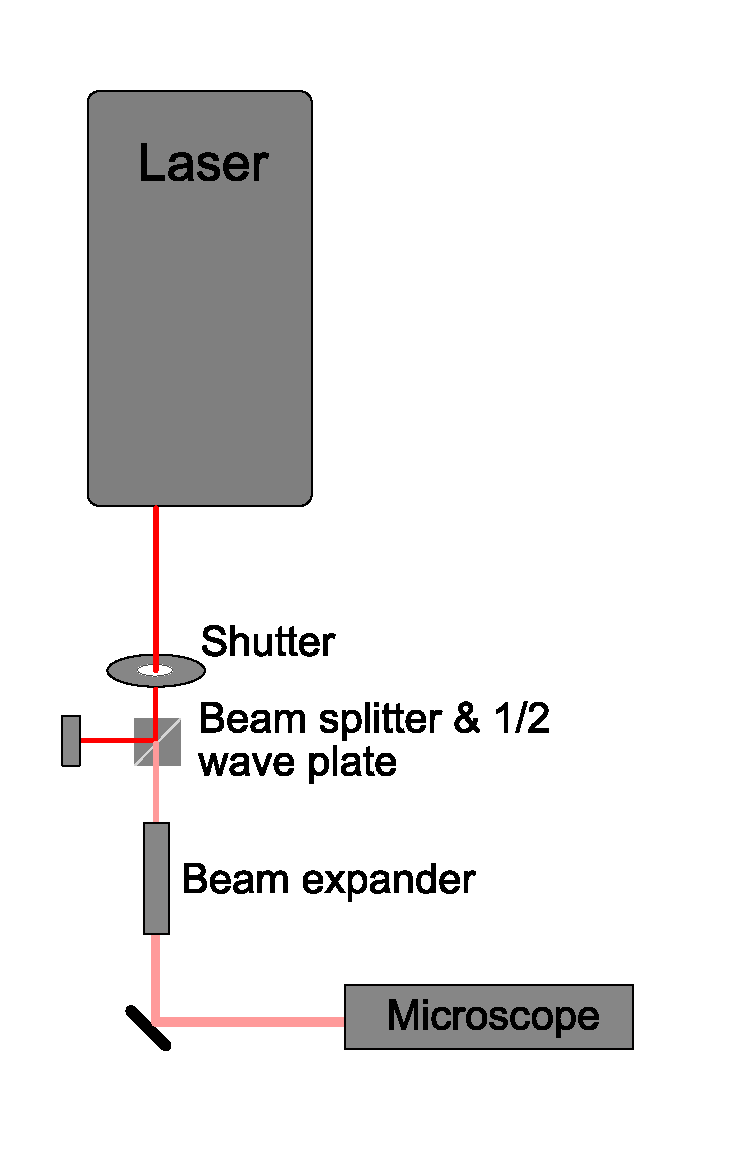
\includegraphics[width=3in]{2p_table_layout.eps}
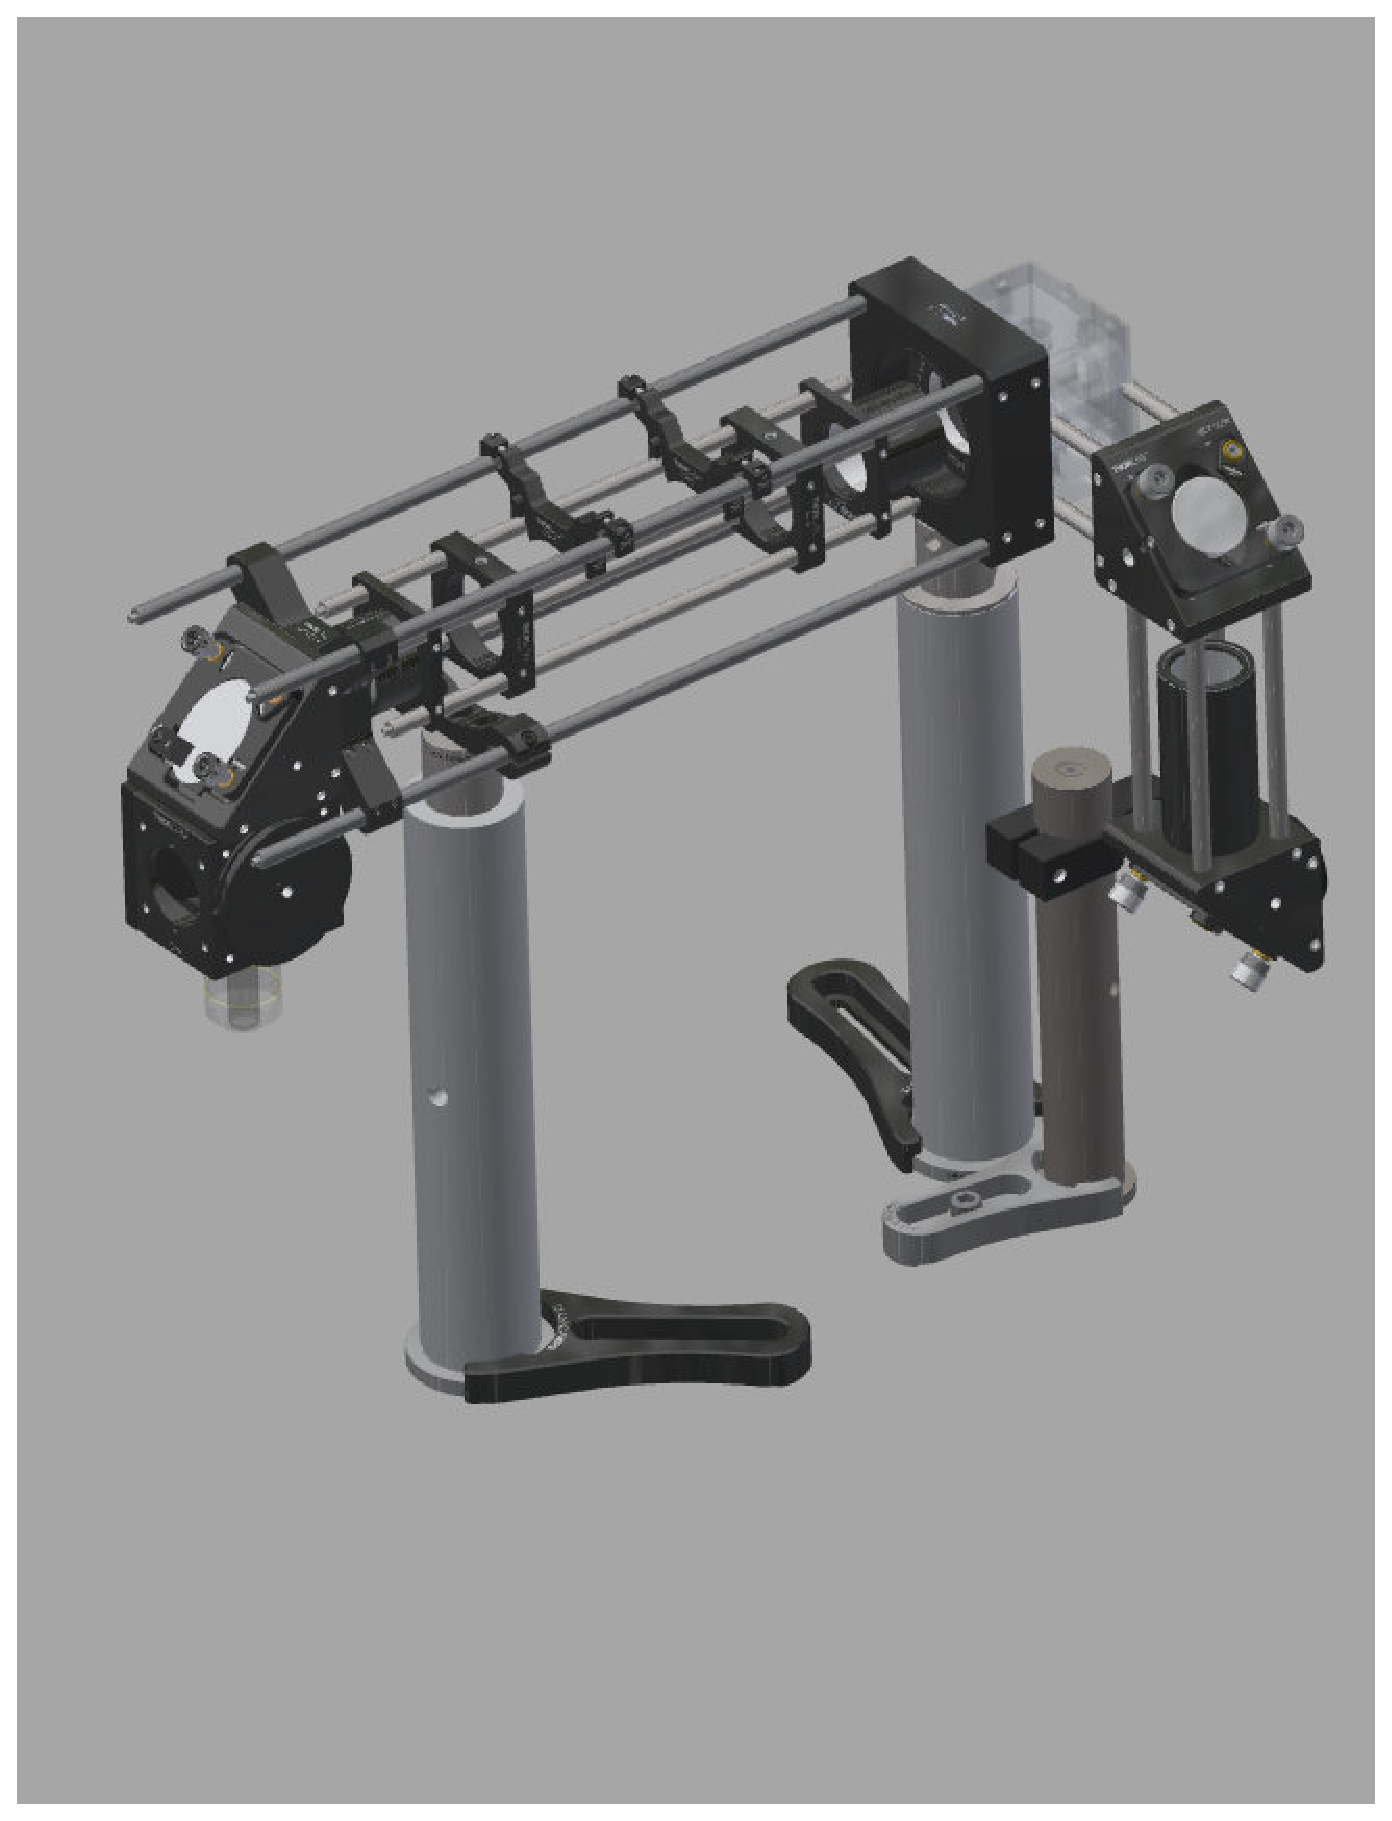
\includegraphics[width=3in]{completed_2p.eps}
\caption{Left: Layout of the main lightpath. Only key components are shown. Right: CAD model of the completed microscope (minus emission detection path).}
\label{fig:layout}
\end{figure}

\clearpage

\subsubsection{Beam Expander}
First you will add the beam expander. 
The completed beam expander is shown in Fig.~\ref{fig:beamExpander}. 
Assemble the expander and place to one side: before inserting it into the light path you will need to think carefully how it will be aligned with the beam. 
The beam will need to travel down the axis of the expander and it will need to emerge collimated.
Avoid touching the lens surfaces and don't force the components together. 

You can check collimation by ensuring the beam doesn't diverge or converge at large distances from the expander. 
You can check alignment by placing two irises on the beam path downstream of where the expander will go and ensuring that the beam is undeviated when the beam expander is put into place. 
Hint: your job will be easier if the beam enters the expander parallel to the table. 

Place a temporary beam block after the telescope for safety.
What is the magnification of the expander and why might we want to expand the beam?

\begin{figure}[h]
\center
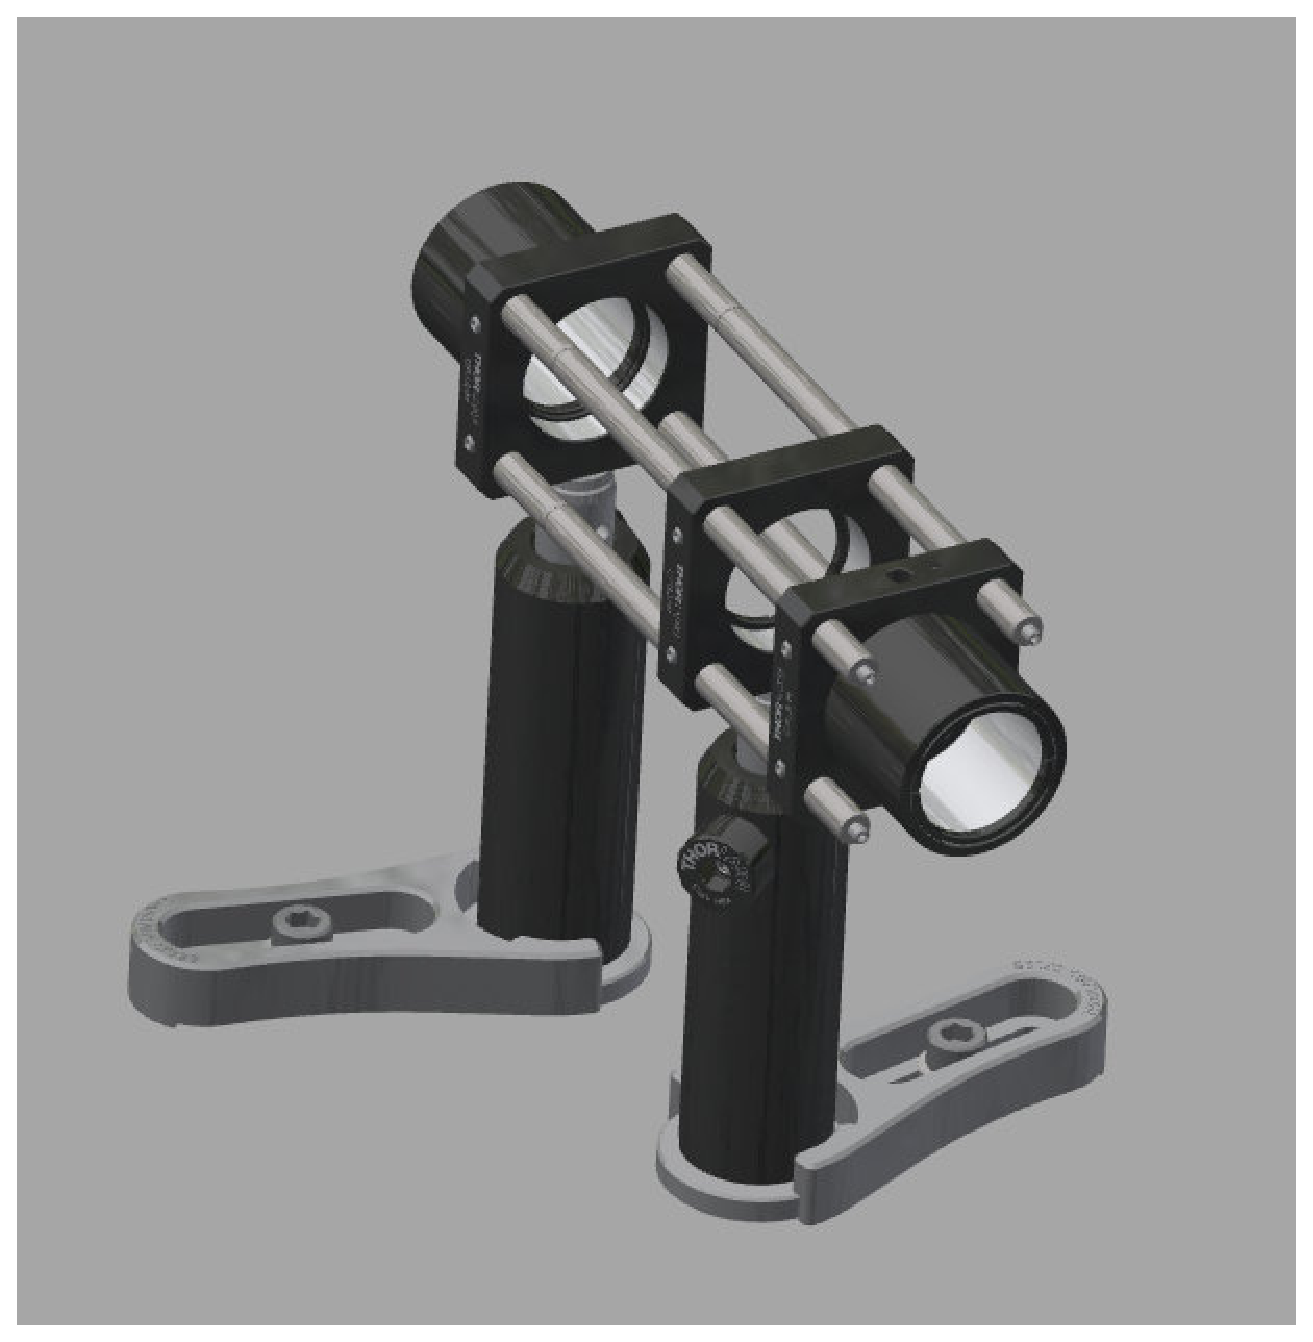
\includegraphics[width=3in]{expander_CAD_01.eps}
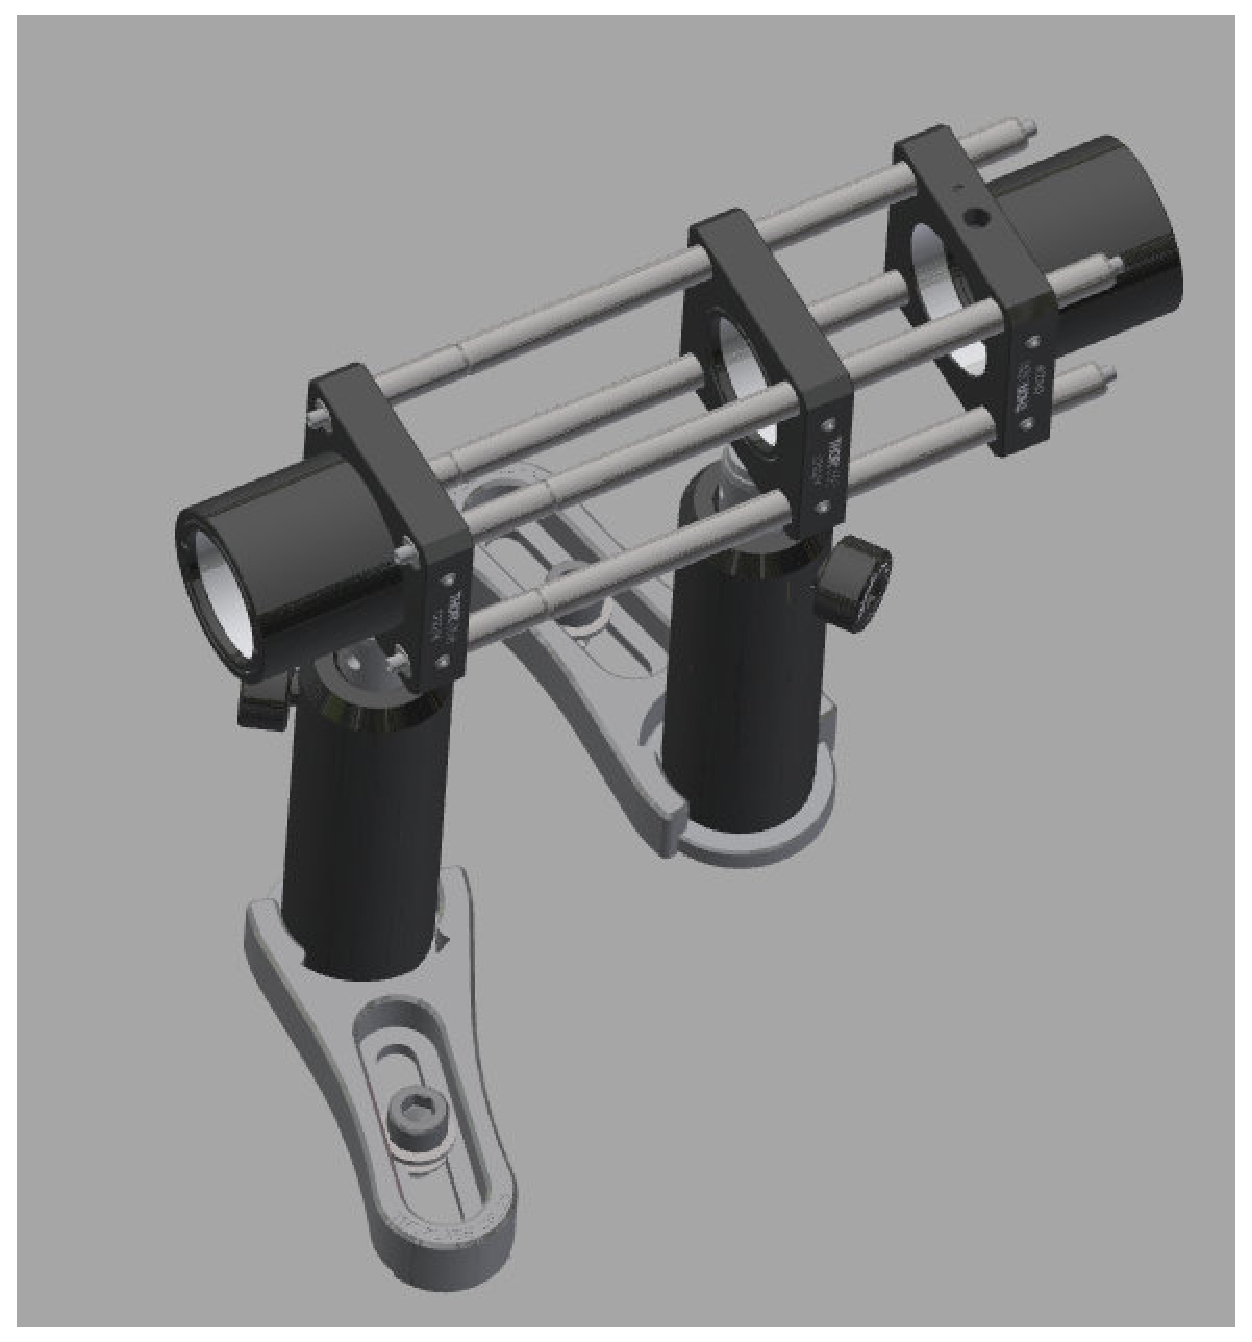
\includegraphics[width=2.85in]{expander_CAD_02.eps}
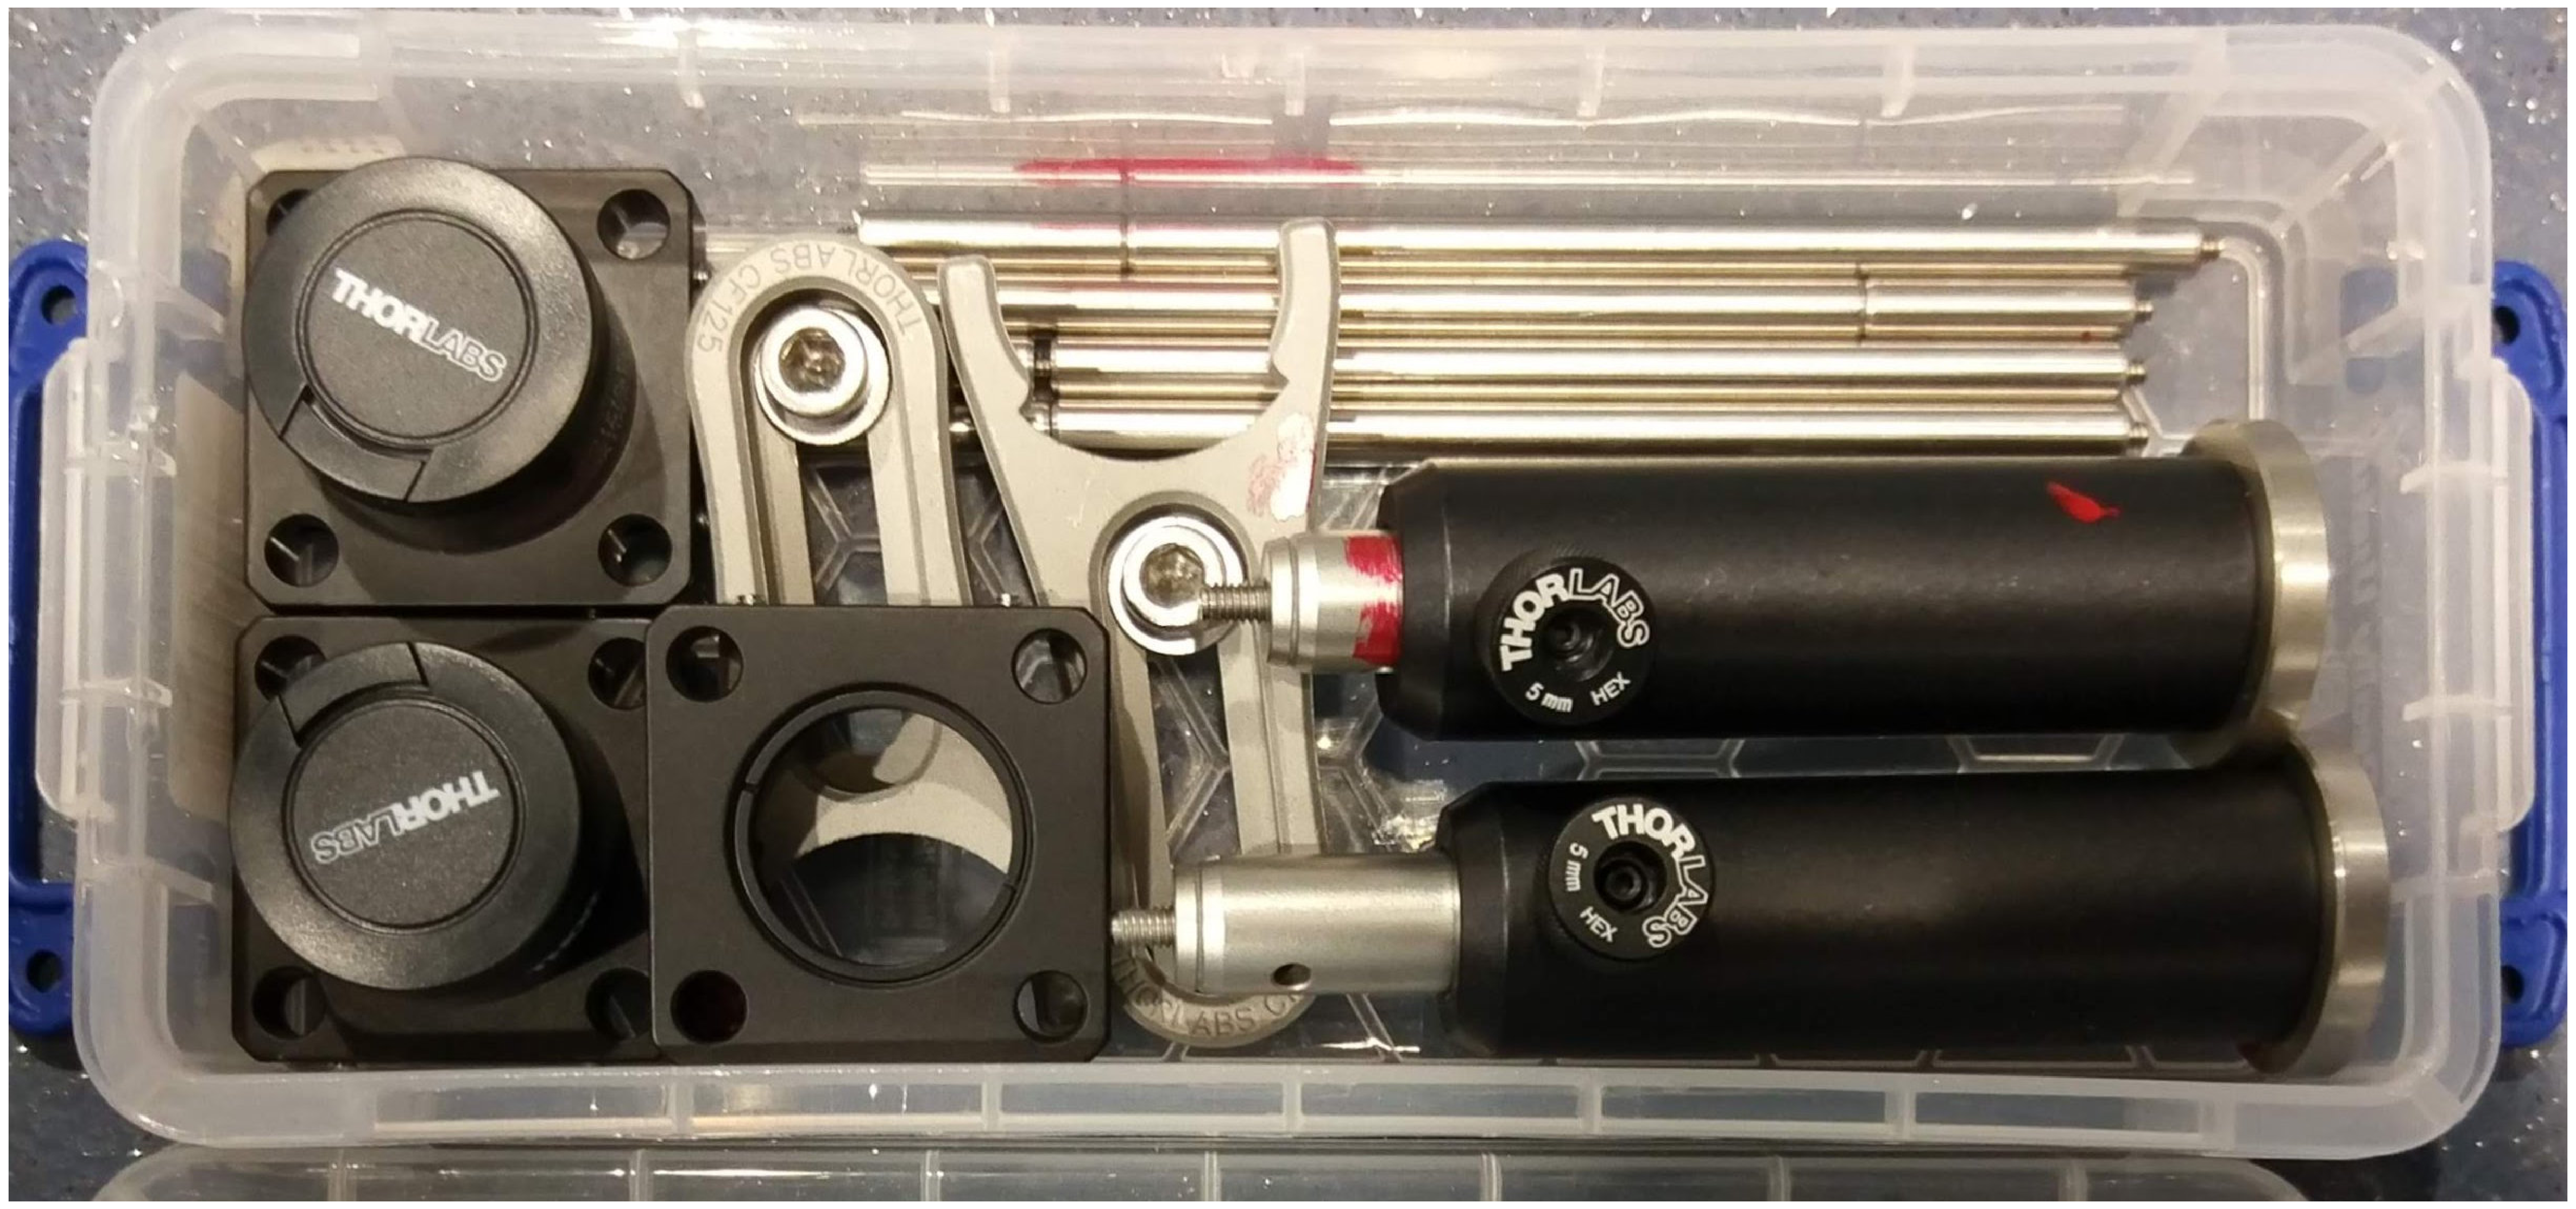
\includegraphics[width=5in]{beam_expander_box.eps}
\caption{Beam expander shown assembled (top) and as components in box (bottom). Avoid touching the lens surfaces.}
\label{fig:beamExpander}
\end{figure}


\clearpage

\subsubsection{Main microscope assembly}
You can now build the skeleton of the microscope frame Fig.~\ref{fig:frame} (left) and mount it on its support pillars Fig.~\ref{fig:frame} (right).
The support pillars, coloured red, are not identical. 
The pillar for the scanner is slightly higher. 
You will find most parts in the box labeled `\textbf{2P Support Mechanics}', which also contains components for supporting the periscope.
The optional SM2 cage plate (shown in purple) is in the 21 L box and can temporarily be used to support the cage if you feel this is necessary. 

\begin{figure}[h]
\center
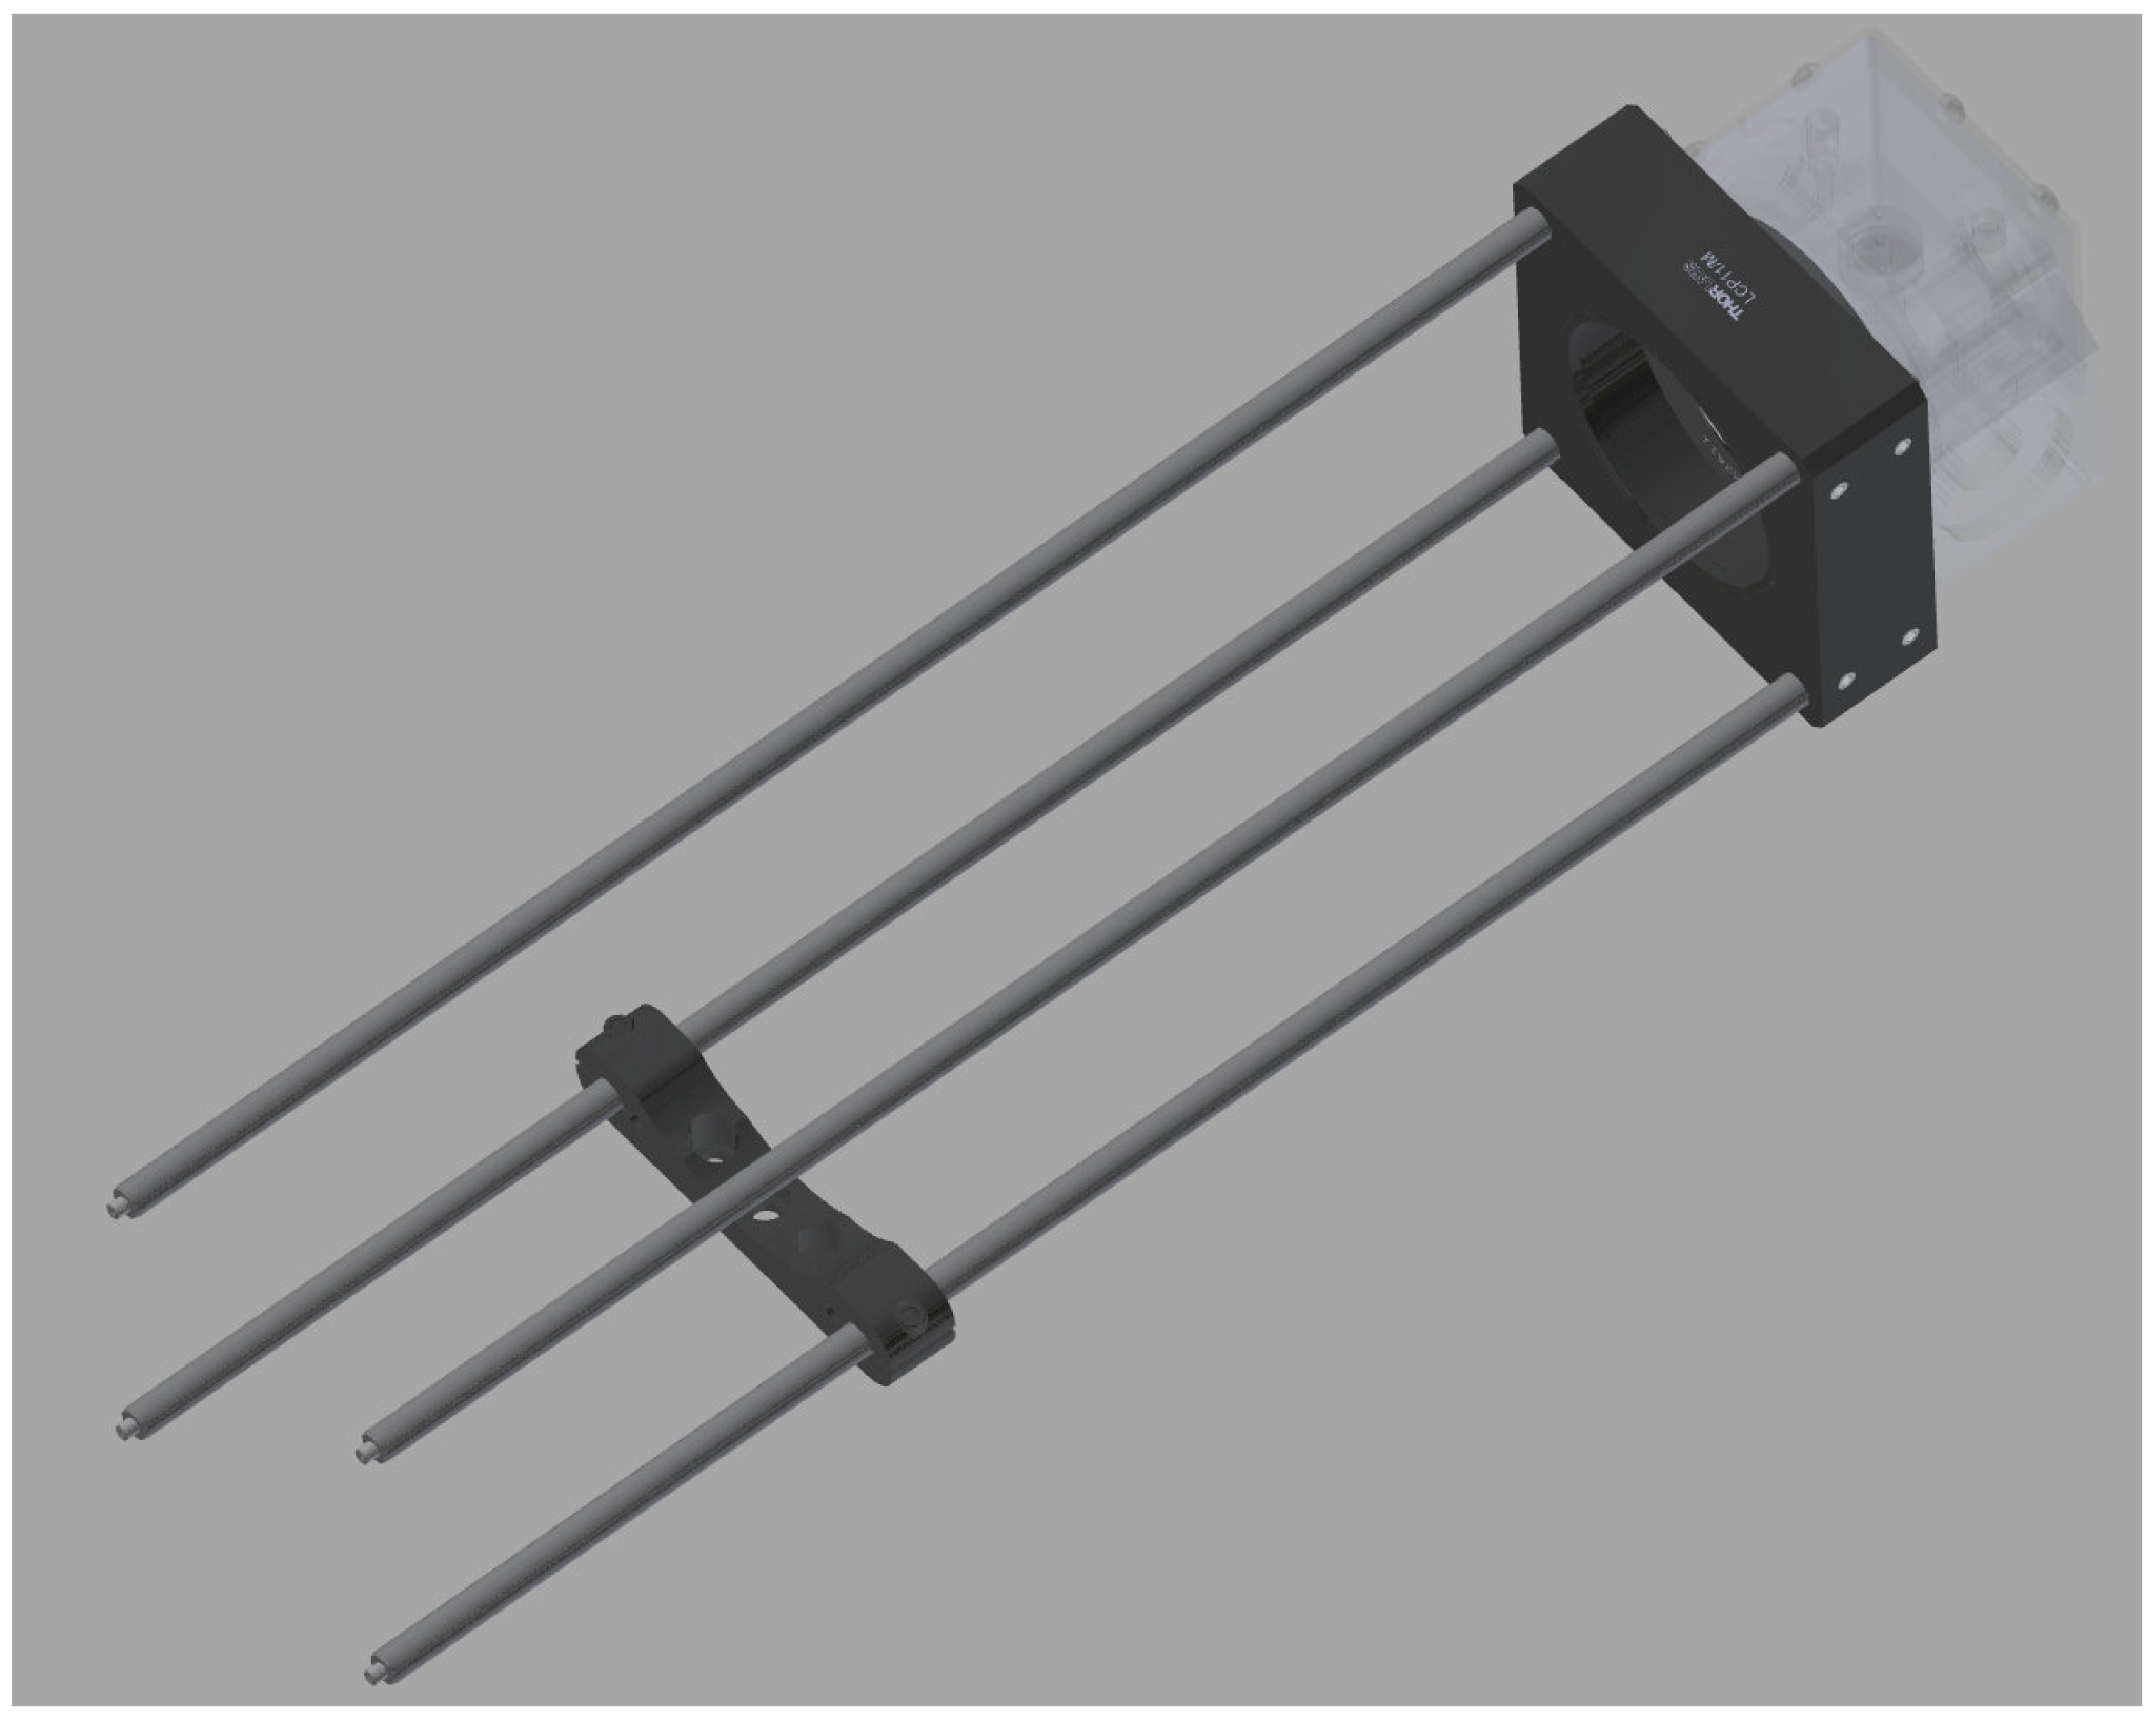
\includegraphics[width=3in]{frame.eps}
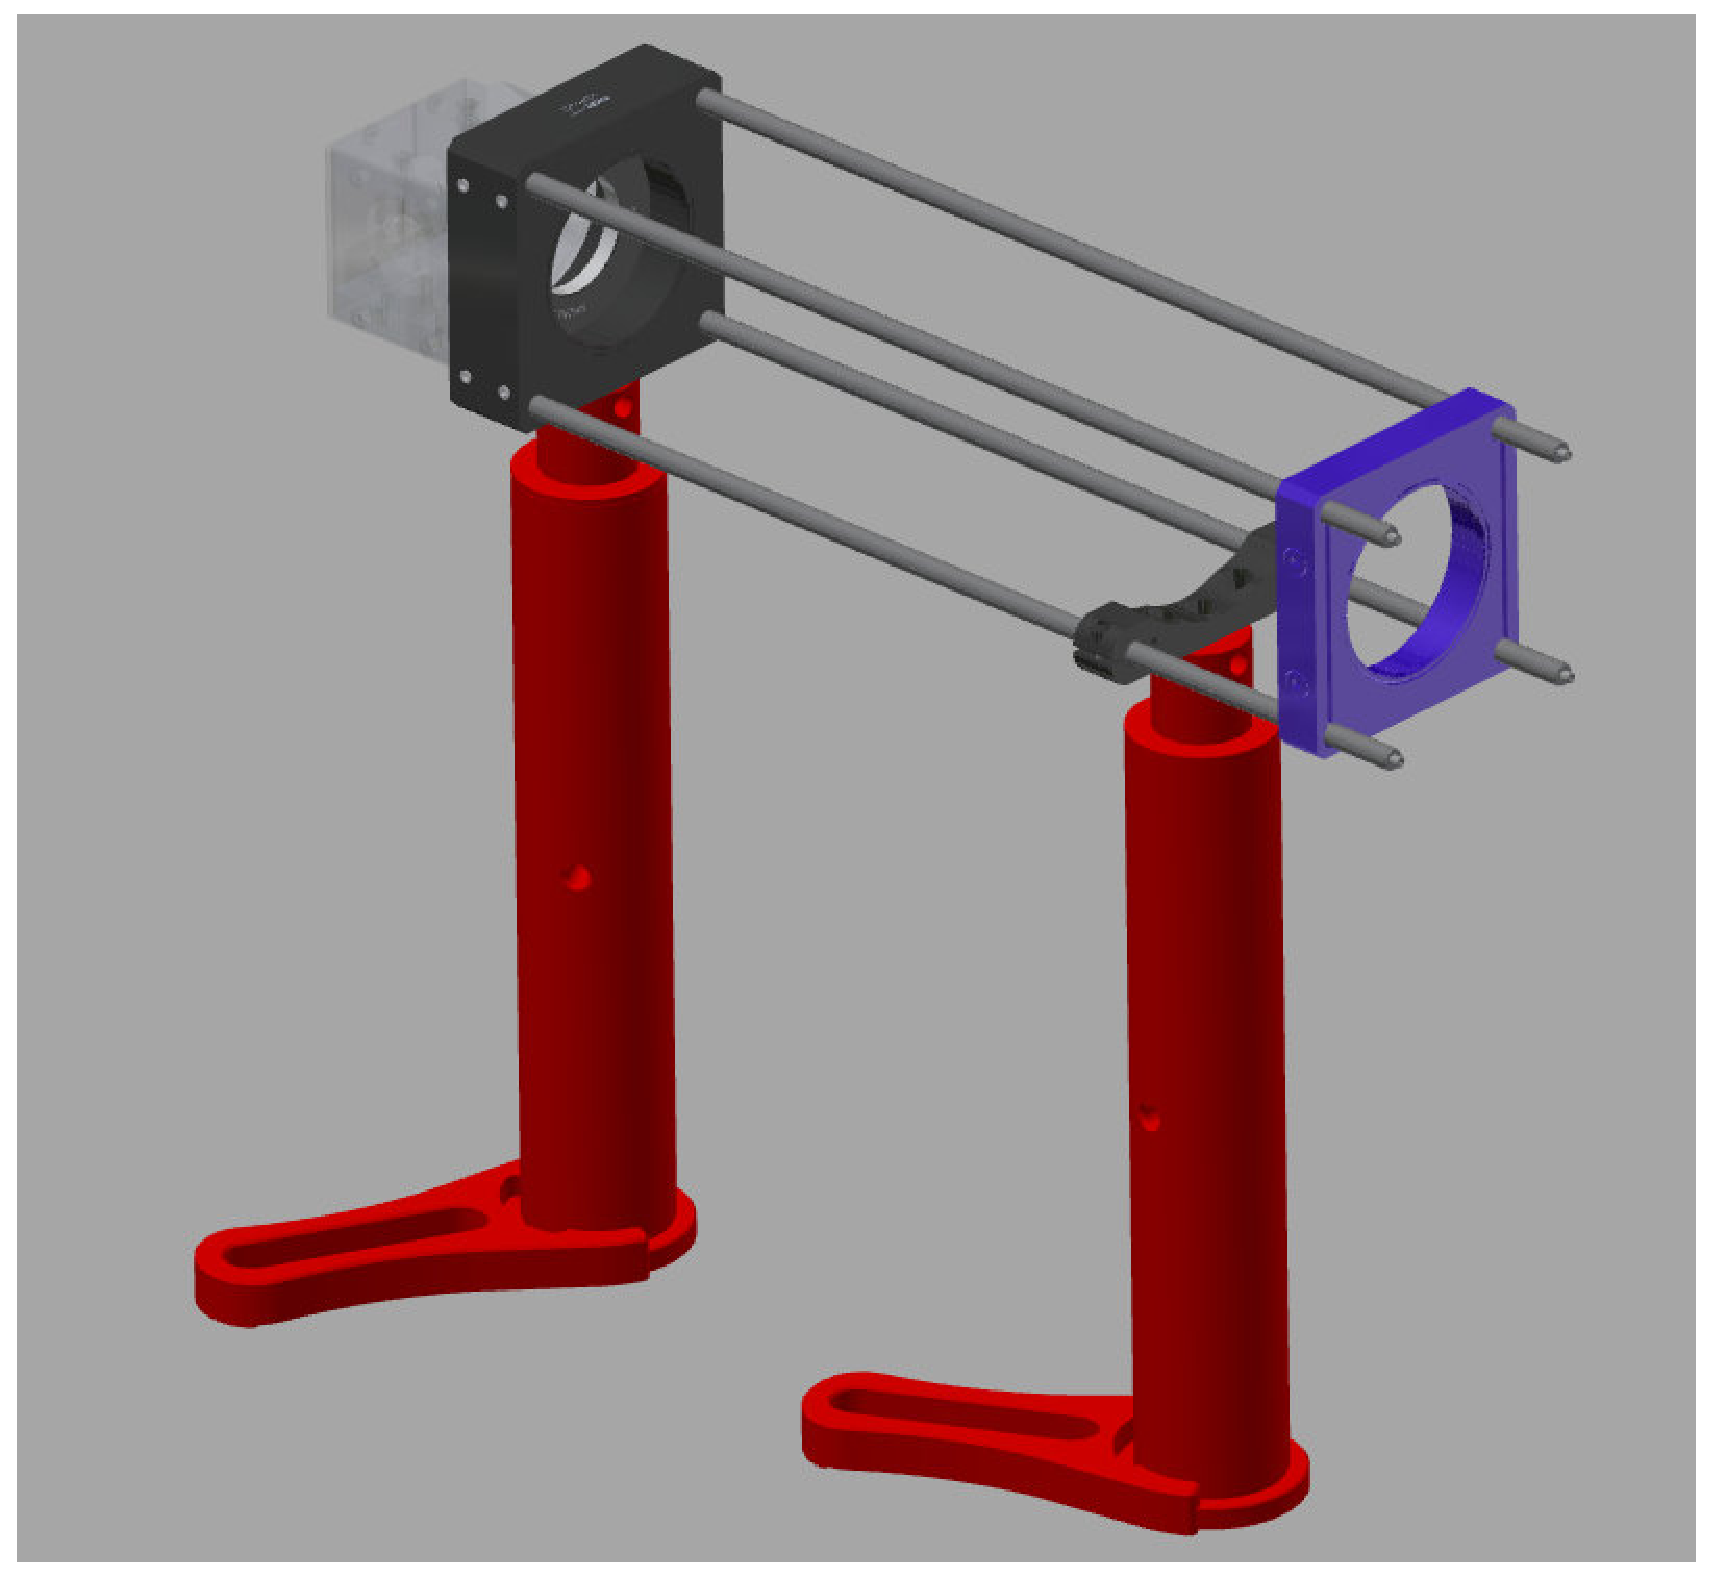
\includegraphics[width=2.61in]{mount_frame.eps}
\caption{Microscope frame (left) alone and mounted on support pillars (right). Support pillars shown in red. Temporary and optional brace for the cage system shown in purple.}
\label{fig:frame}
\end{figure}

\subsubsection{Periscope}
The periscope brings the beam up into the scan head. 
Assemble the parts in the `\textbf{Periscope}' box such that they look as shown in Fig.~\ref{fig:periscope}. 
Depending on how the light path is arranged you might wish to alter the orientation of the upper and lower mirrors. 
There is an extra alignment iris in the periscope box, you can place this wherever you think is most helpful.
You can now attach the periscope to the microscope and support it with the components shown in red. 
You will find those in the box labeled `\textbf{2P Support Mechanics}'.
Ensure the periscope is vertical and not tilted and that the scanner enclosure is square with respect to the cage system. 
Once bolted to the table, the periscope will also stop the scanners from rotating in the SM2 cage plate to which they are screwed.
\textbf{Do not tighten the scanner hard onto the connected cage plate: it can jam. Be gentle.}


\begin{figure}[h]
\center
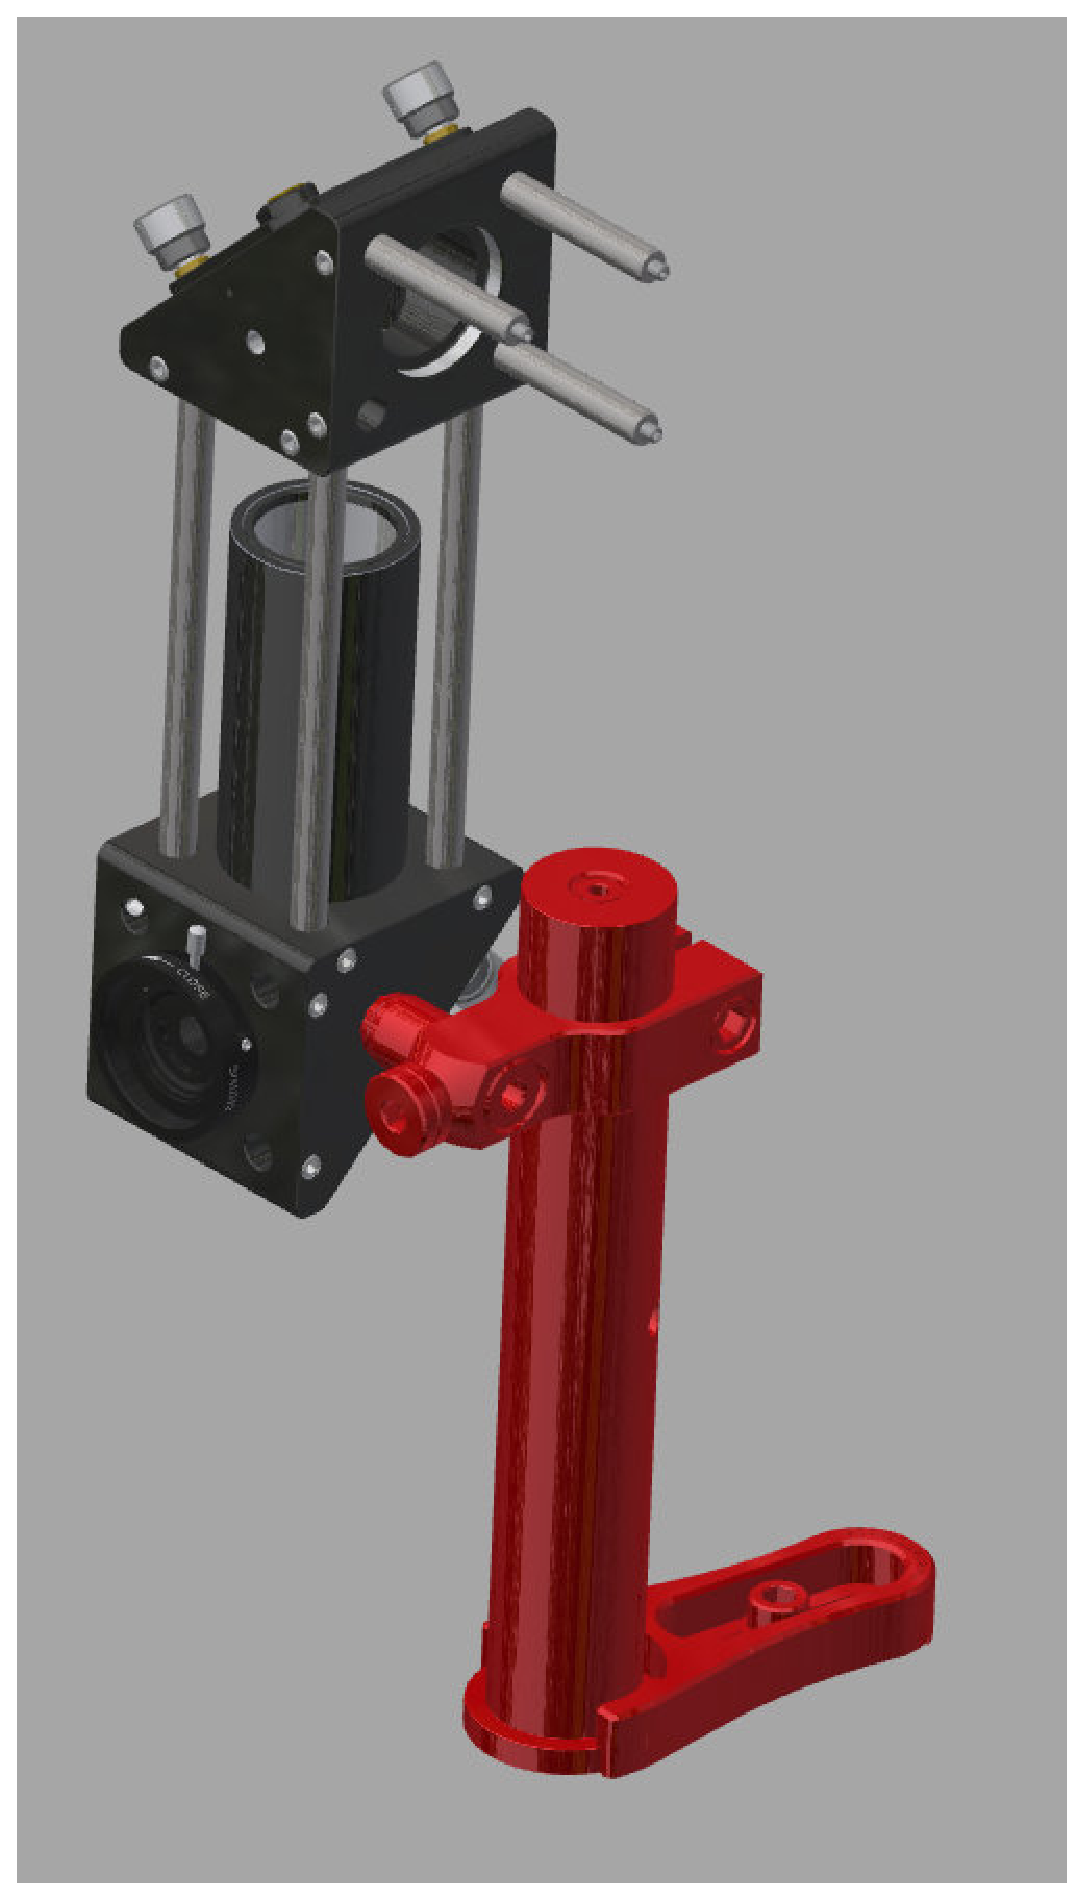
\includegraphics[width=1.5in]{periscope_01.eps}
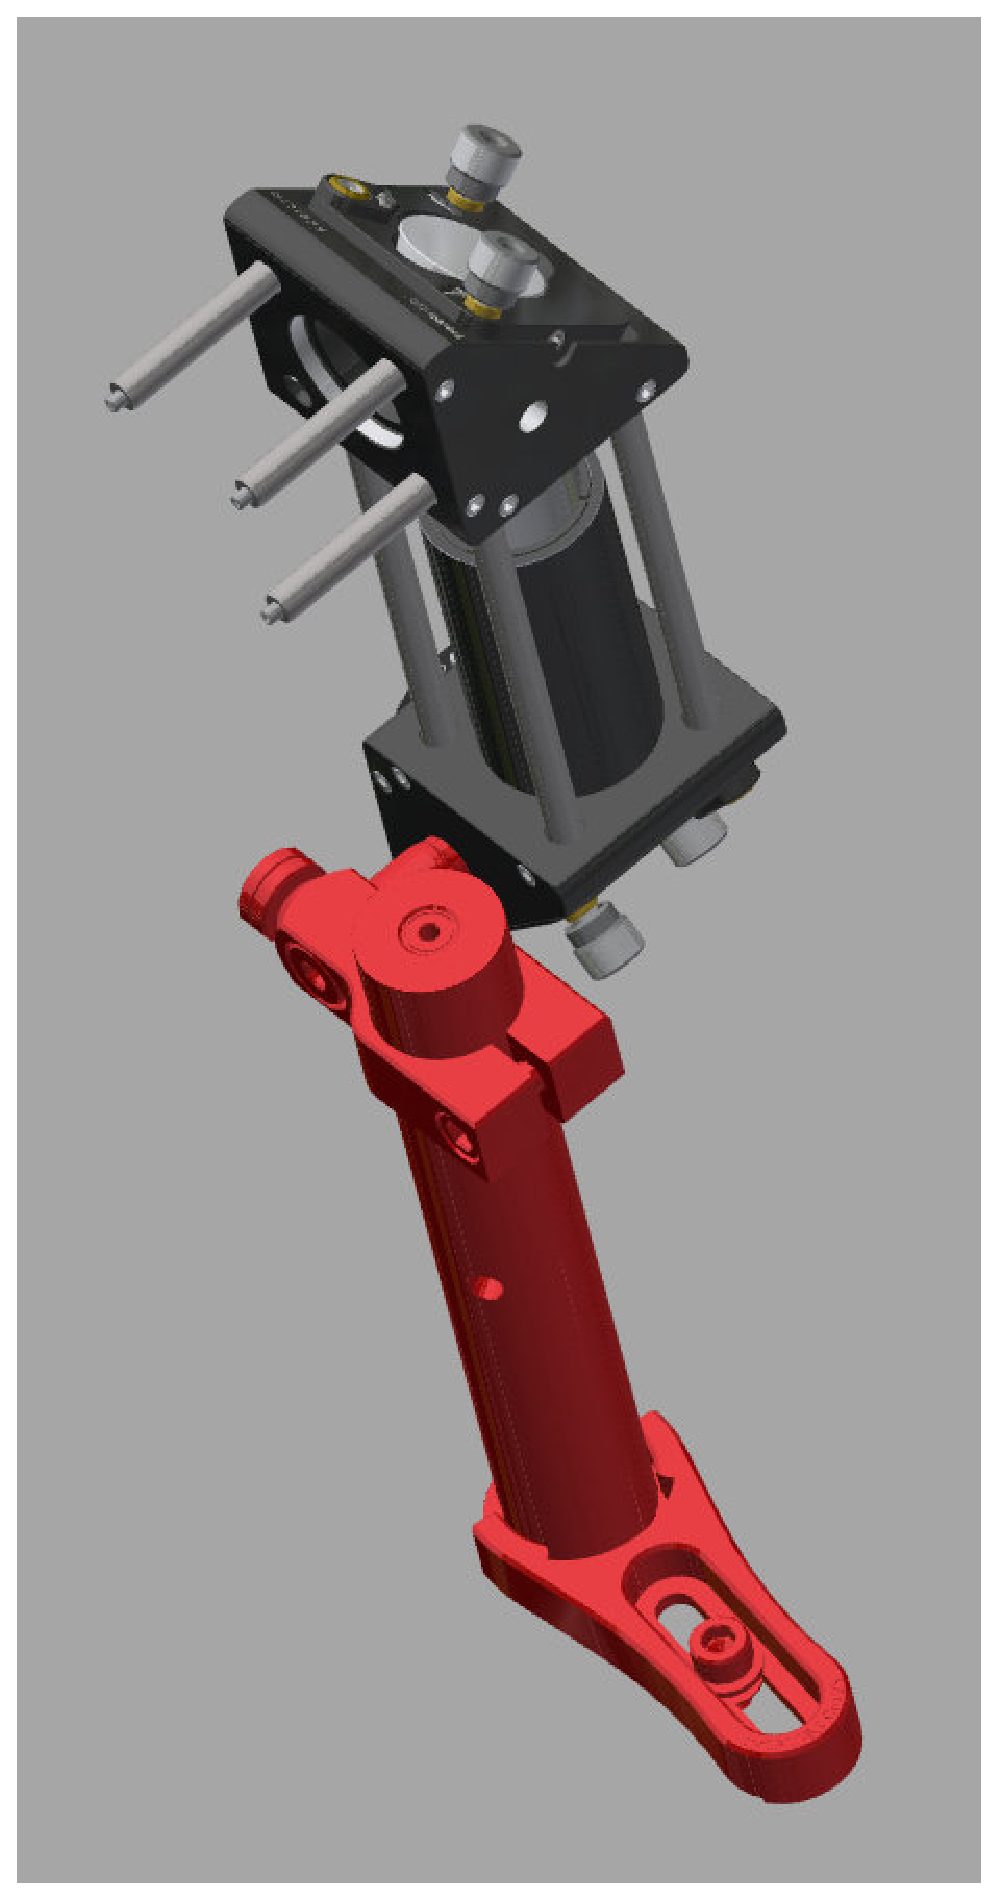
\includegraphics[width=1.38in]{periscope_02.eps}
\caption{Periscope assembly. Support structures shown in red.}
\label{fig:periscope}
\end{figure}


\clearpage

\subsubsection{Aligning the beam with the frame}
You are now in a position to feed the the beam into the scanners. 
\textbf{Be cautious feeding the beam into the periscope: perform this step with assistance}. 
Use the provided alignment tools and your beam alignment skills to get the beam traveling straight down the middle of the microscope frame. 
\textbf{Before beginning, ensure the scanners are powered and zeroed. Always be aware of where the beam is located.}

\subsubsection{Scan Optics}
You will now assemble the scan lens and tube lens module. 
The parts you will need are in the box labeled `\textbf{2 Photon Scan Optics}' and are to be assembled as shown in Fig.~\ref{fig:scan_optics}.
Avoid touching the lens surfaces. 
Once assembled, you can drop the unit into the microscope frame. 
Ensure the beam exits the assembly collimated. 
Take care with the CDA1 drop-in hangers: tighten gently and only once they are clamped onto a rod.
What is the total expansion of the beam?



\begin{figure}[h]
\center
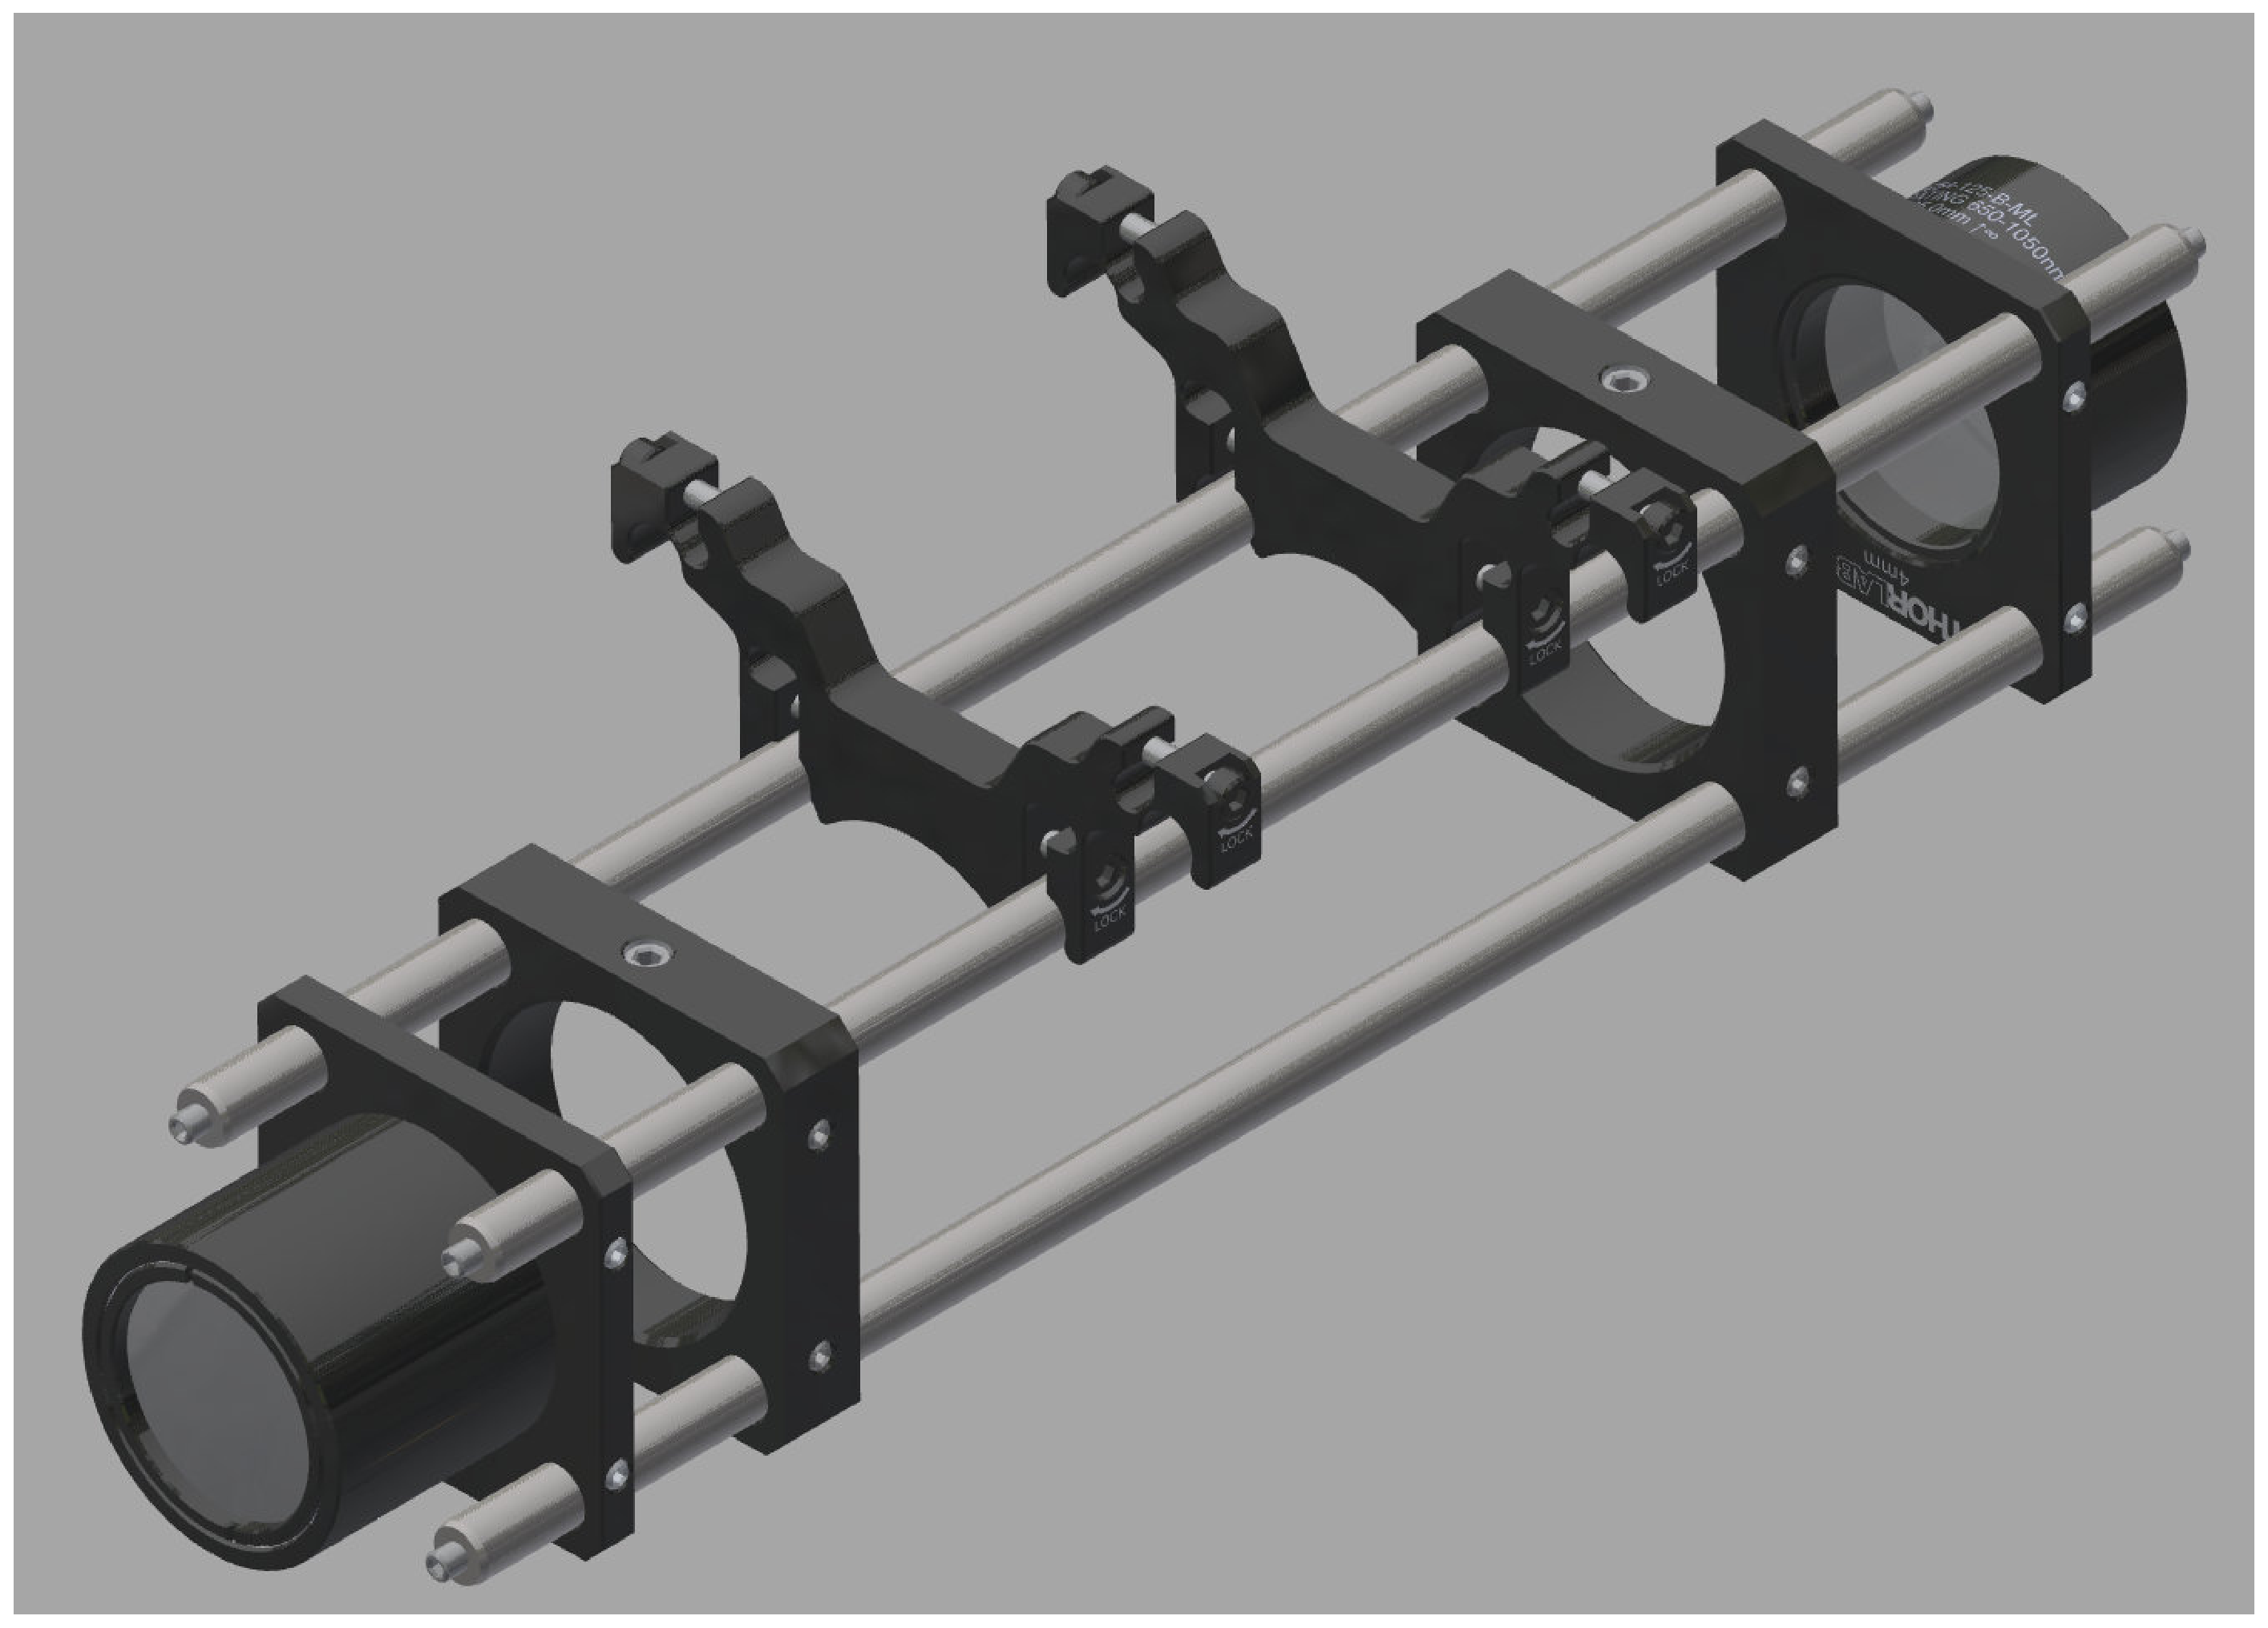
\includegraphics[width=4.5in]{scan_optics_01.eps}
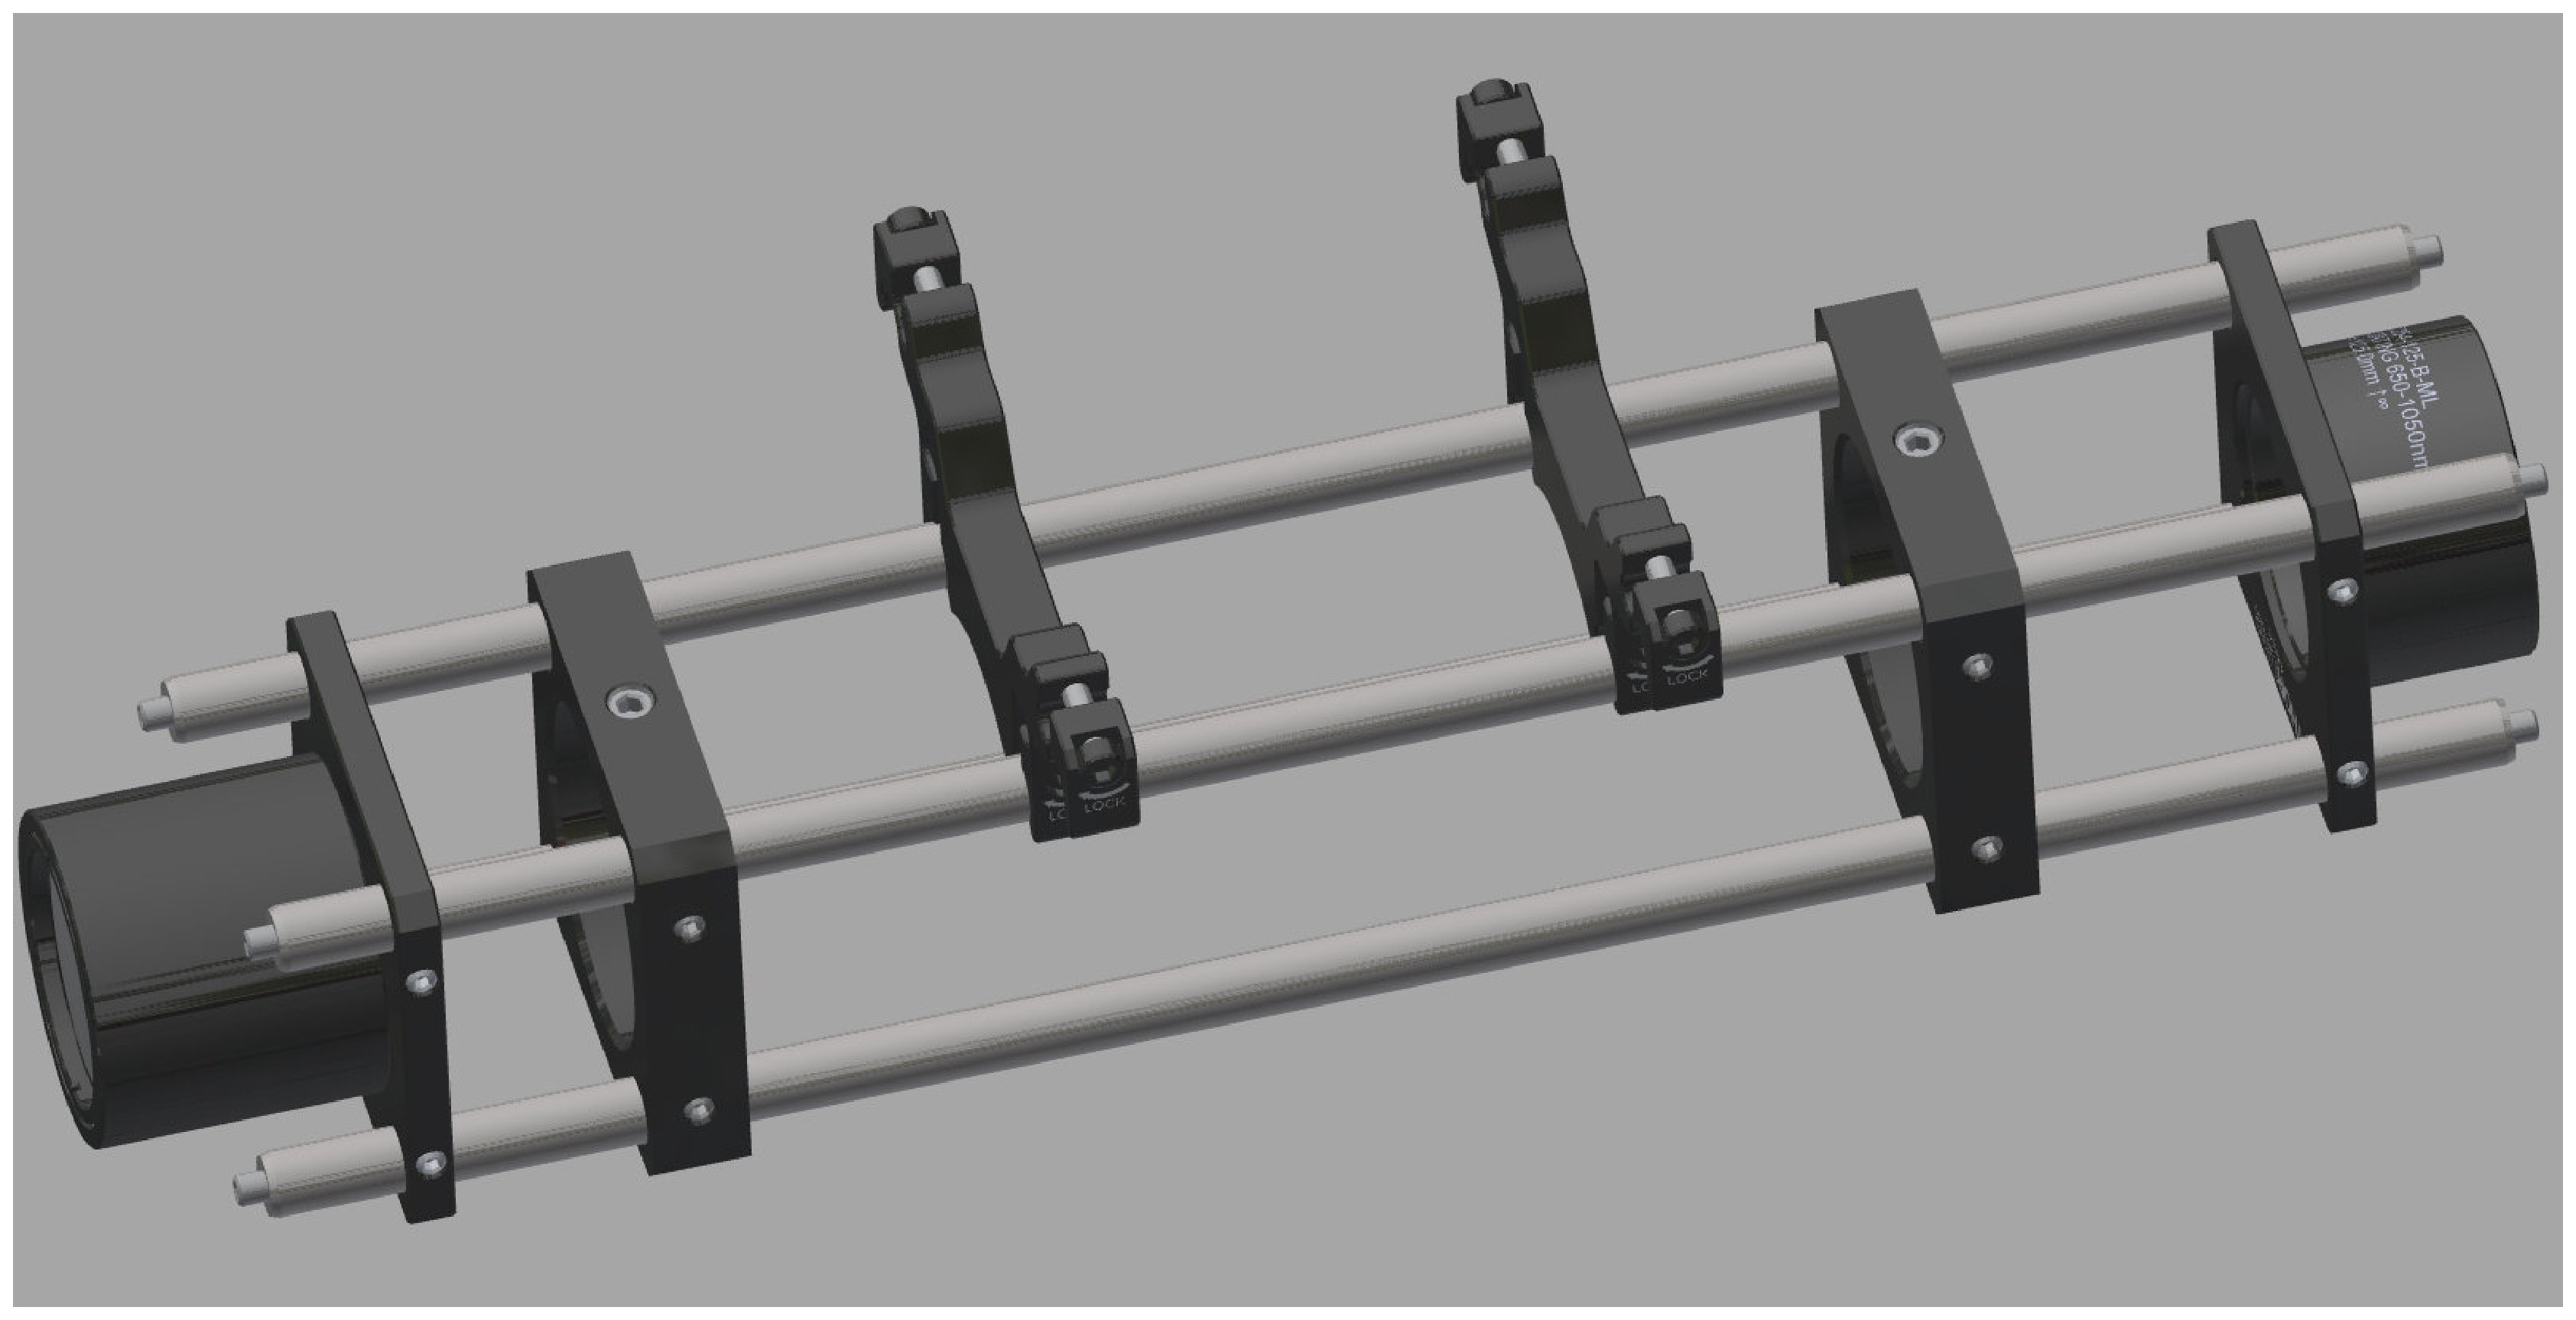
\includegraphics[width=4.5in]{scan_optics_02.eps}
\caption{Scan and tube lens module.}
\label{fig:scan_optics}
\end{figure}

\clearpage

\subsubsection{Completing the excitation path}
If you had an SM2 cage plate (the one highlighted in purple) supporting the frame, you will need to remove it to add the dichroic cube (Fig.~\ref{fig:dichroic_holder}).
Think before you do this, however. 
How far should the scanner relay optics be from the scanners and how far from the tube lens should the dichroic cube be mounted?
The path of the beam through the cube is depicted in Fig.~\ref{fig:dichroic_holder} as a red line.
To help you with this step, you can move the scanners over a small scan angle whilst looking at the the beam motion. 
Use ScanImage for this, as it is has been configured to avoid large scan angles.
\textbf{Be cautious: the beam might still spill out of the scan head. Stand behind the scanners and perform this step with assistance}.
Finally, is the beam exiting the cube traveling directly downwards and so on-axis with the objective we will add?
Use two rods and the spring-loaded SM1 target to check. 

\begin{figure}[h]
\center
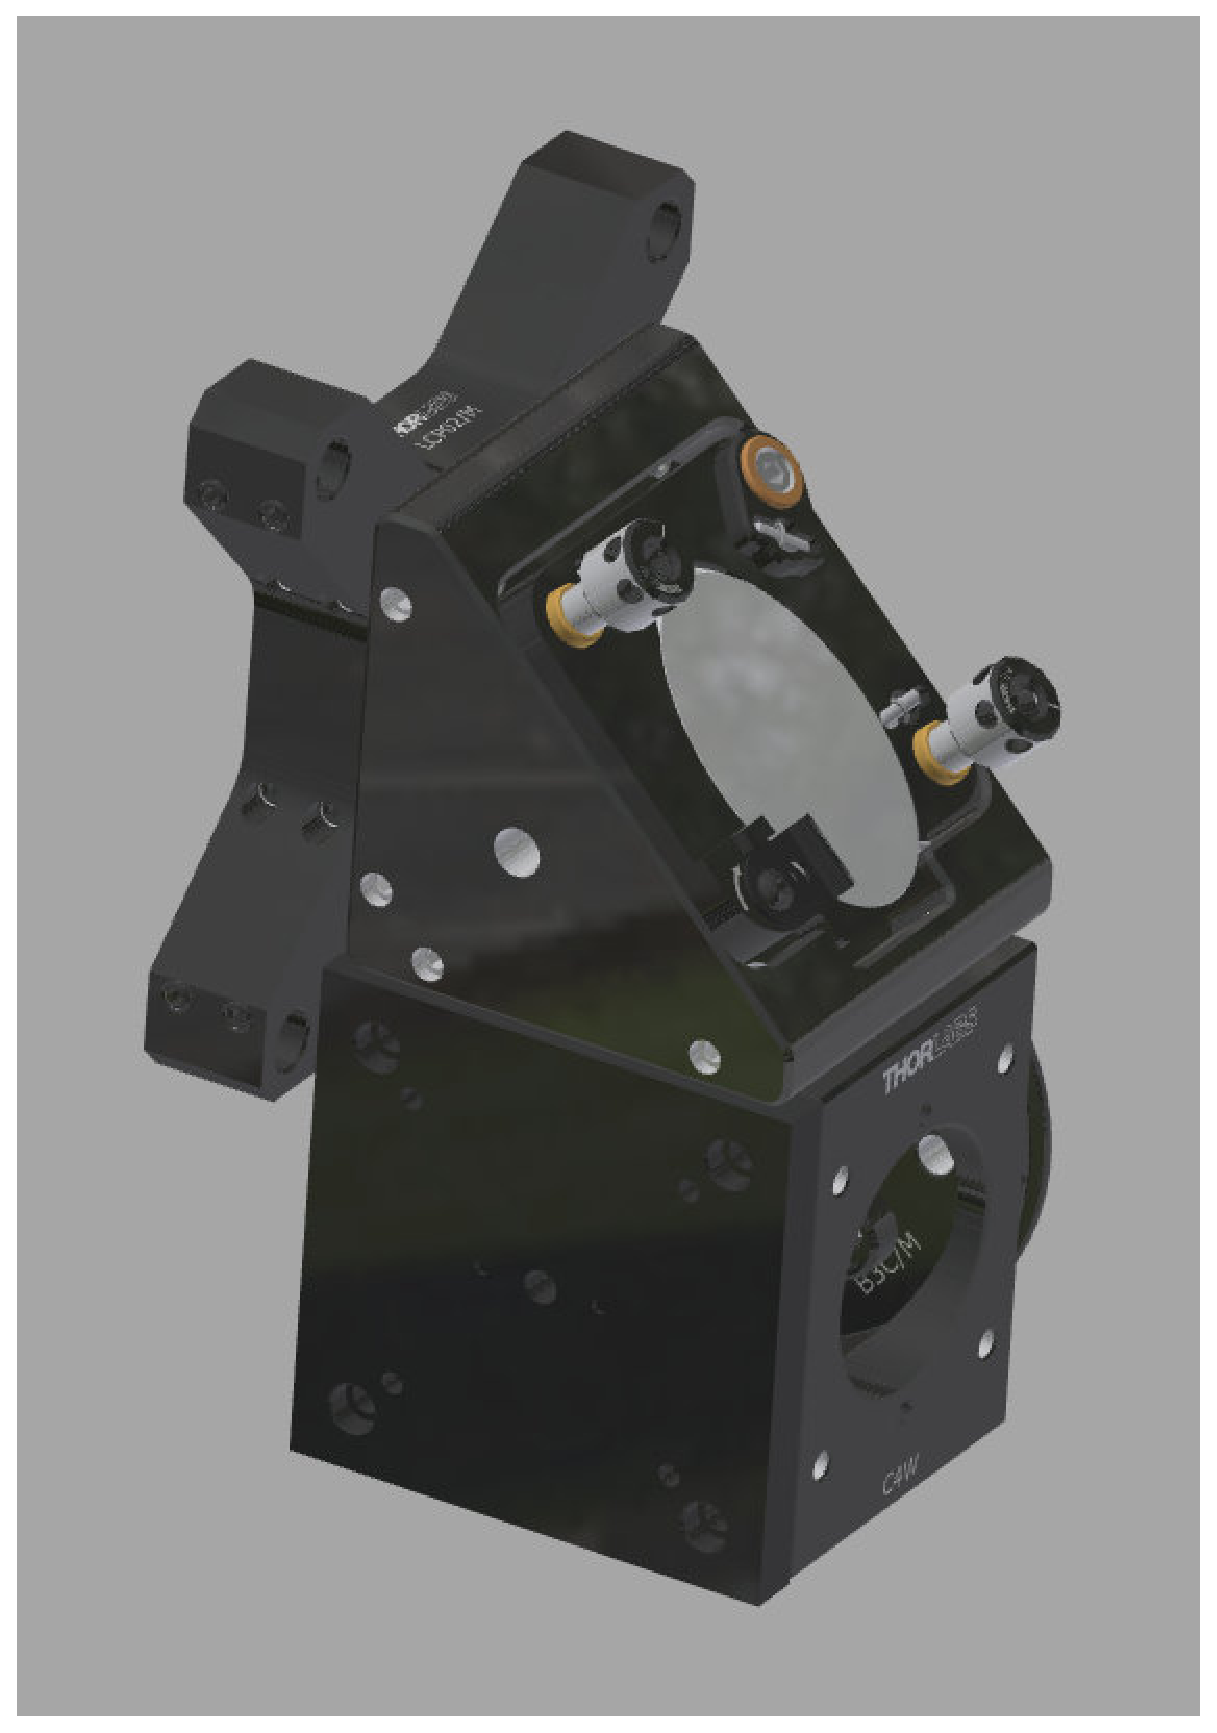
\includegraphics[width=2.0in]{dichroic_cube.eps}
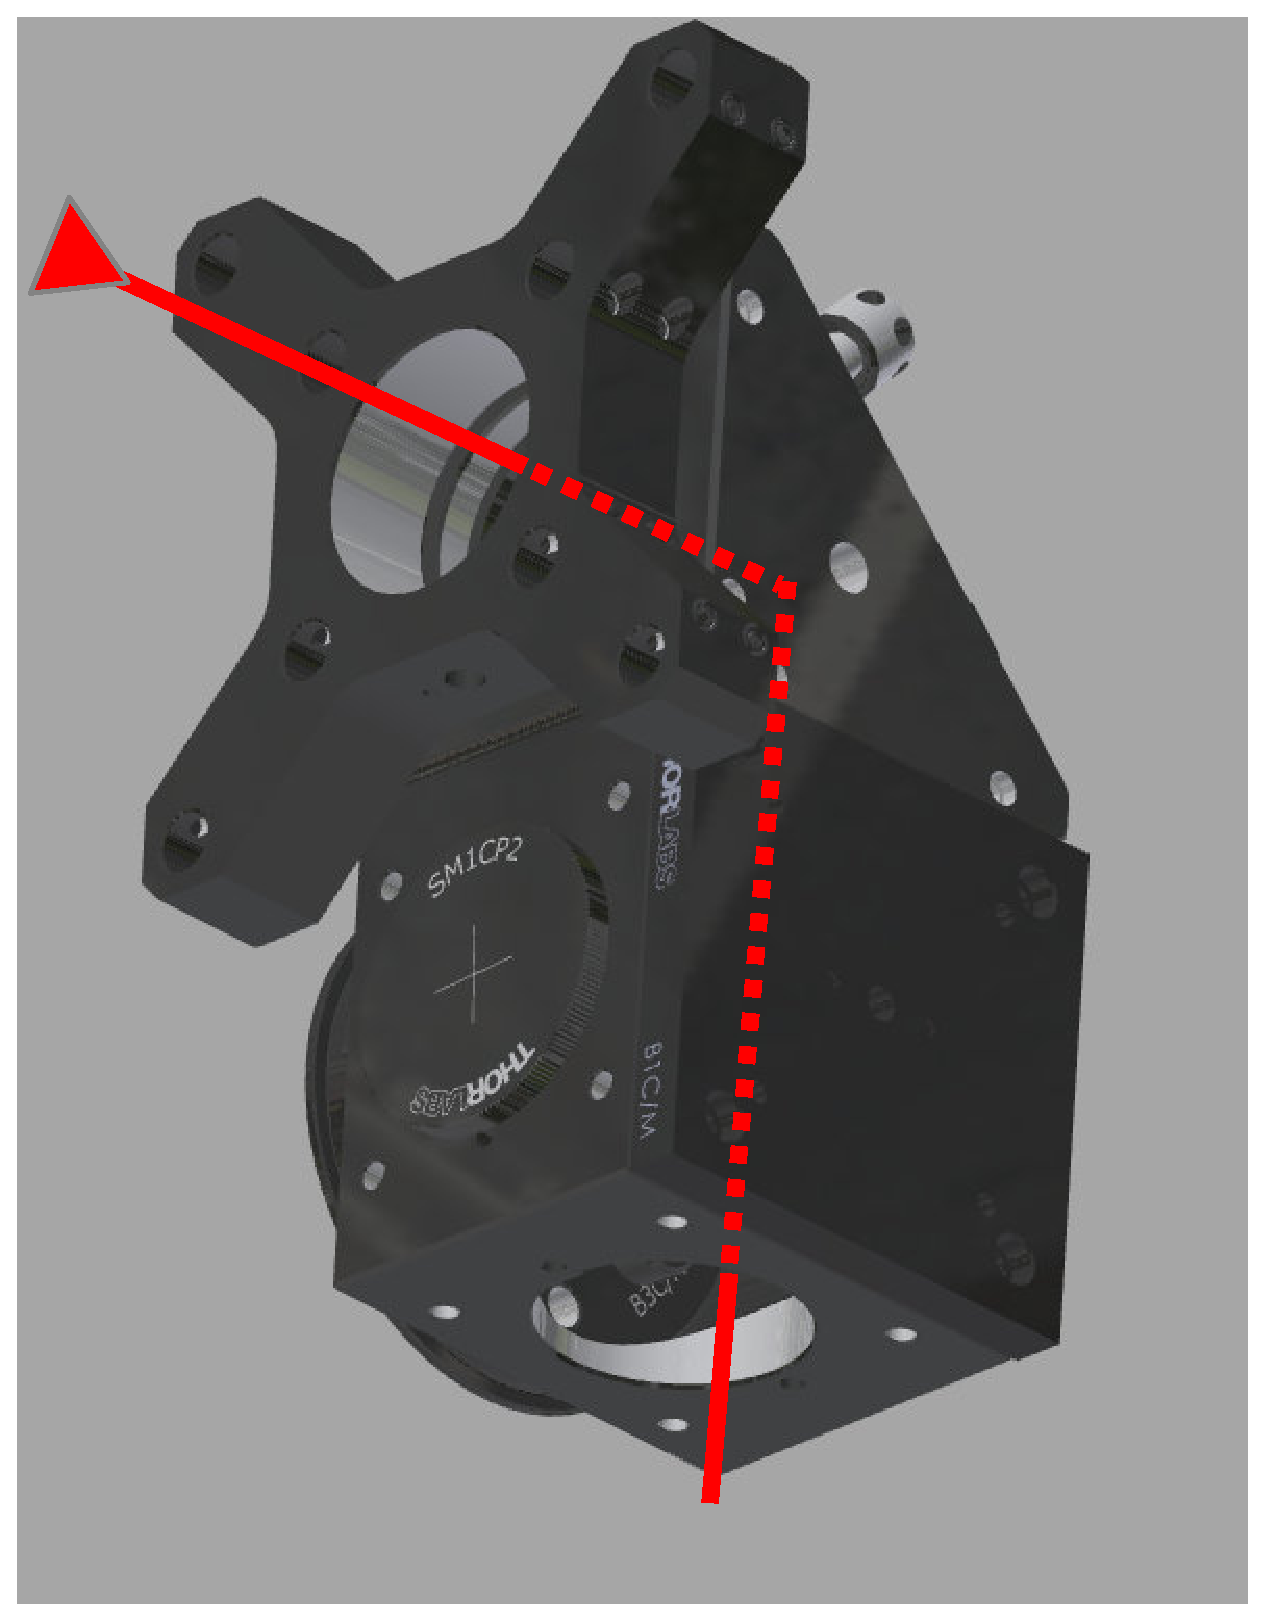
\includegraphics[width=2.0in]{laser_path_through_cube.eps}
\caption{Dichroic cube. Image on the right shows the path of the laser beam through the component.}
\label{fig:dichroic_holder}
\end{figure}


Once you are satisfied with the alignment, you can try scanning a fluorescent plastic sample card and confirming by eye that you get fluorescence whilst the beam is moving over the sample:
\begin{itemize}
    \setlength\itemsep{0.15em}
     \item Insert the 40x objective.
     \item Add the 3-axis stage under the objective.
     \item Place a Chroma fluorescent sample card on the stage and carefully bring it up to the objective. Working distance is 2 or 3 mm. 
     \item Use water as the immersion medium.
     \item Use a low laser power and a suitable wavelength. 
     \item Start scanning and focus until you see fluorescence.
 \end{itemize}

\clearpage

\subsubsection{Adding the emission path}
You now have a functioning excitation path, but you need a detector in order to get an image. 
You will now to add a PMT with appropriate relay optics in order to capture the fluorescence on the PMT surface. 
A schematic depicting the path the emitted light will take is shown in Fig.~\ref{fig:dichroic_holder_paths}.
Think carefully what lens or lenses you need to add before the PMT. 
Hint: what should be conjugate with the PMT?
What other optical element do you need to add before the PMT?

The PMT is \textbf{delicate}. 
Do not expose it to even room light when powered on, as this will damage the photocathode. 
Get assistance to power the PMT and hook up the amplifier. 
\begin{figure}[h]
\center
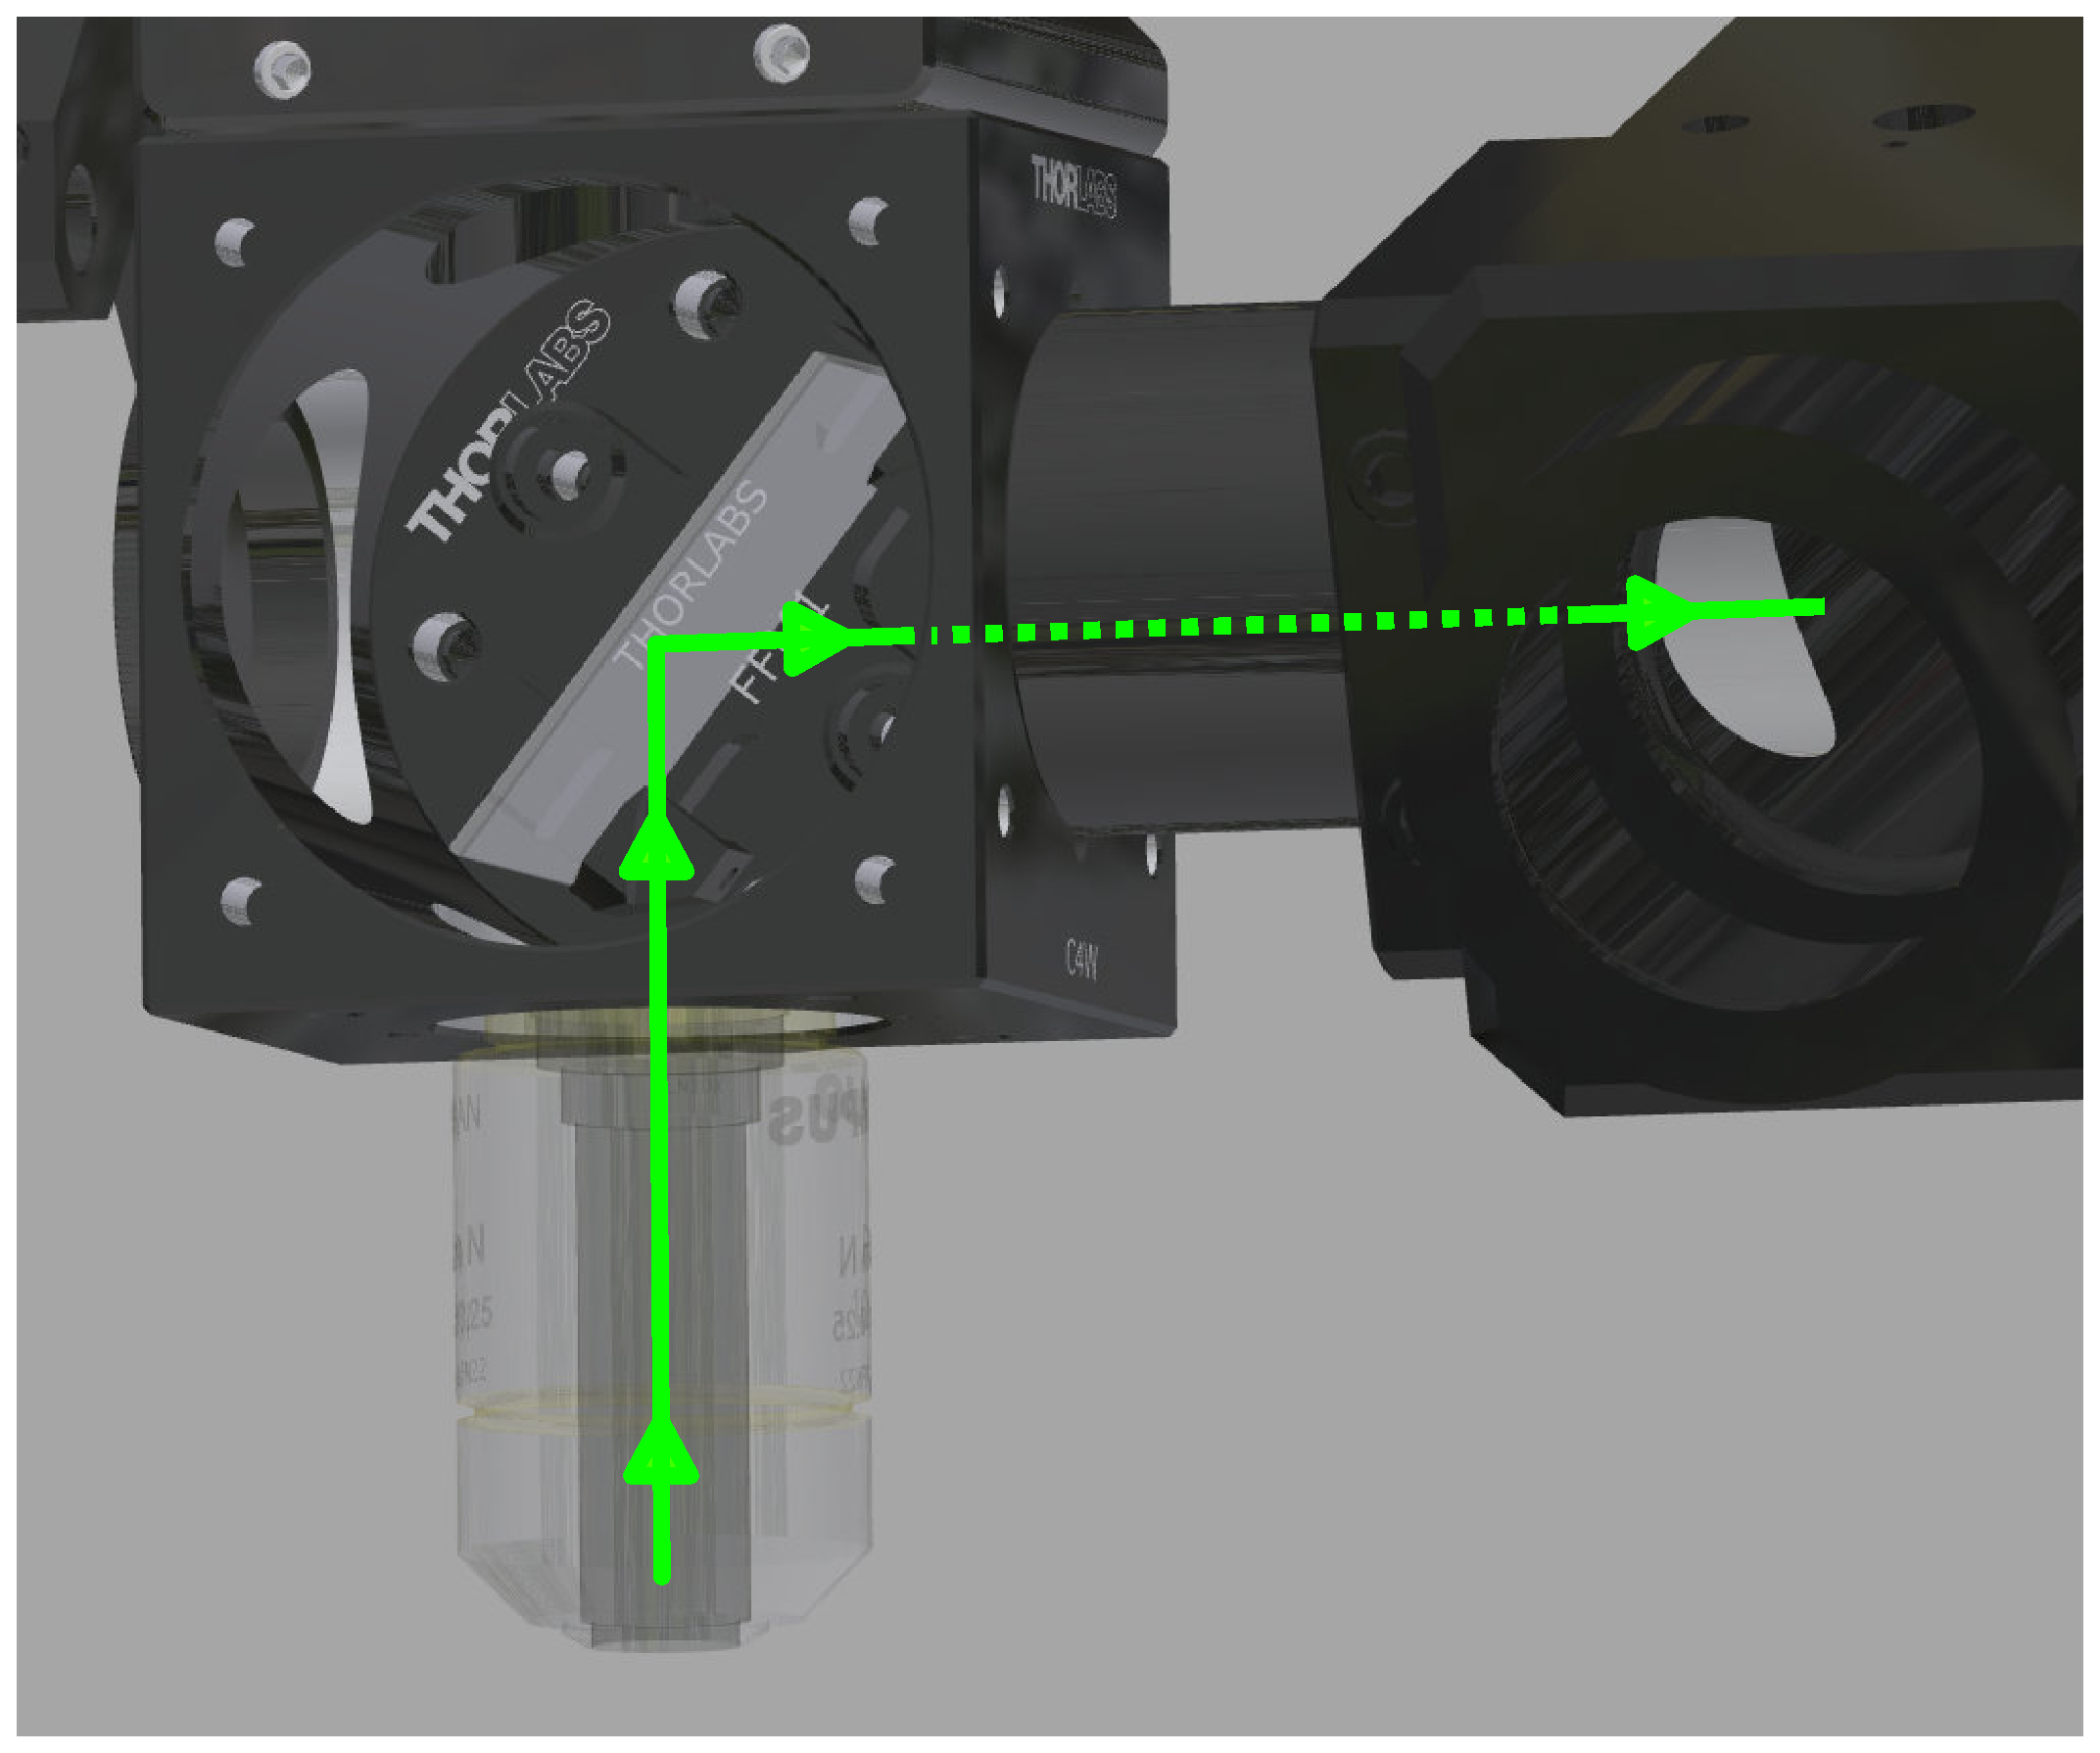
\includegraphics[width=3.1in]{cube_emission_cutout.eps}
\caption{Path of the emitted light through the dichroic cube. The cube's side-plate is removed to show the dichroic mirror itself. The illustration also shows the objective (transparent) and PMT holder (to the far right).}
\label{fig:dichroic_holder_paths}
\end{figure}


\subsubsection{Obtaining an image}
Time to obtain some images!
\begin{itemize}
\item Image the fluorescent sample card. 
\textbf{Use low laser power as this sample is very bright}. 
Use 1x zoom. 
This sample provides information on how uniform the illumination is.

\item Image the $25~\mu m$ pitch copper EM grid at 1x, 2x, and 3x zoom. 
How many microns per pixel do you get?
Use any wavelength at low power. 

\item Image some pollen grains. 
Try focusing up and down through them to get a feeling for the optical sectioning ability of your microscope. 
The micrometer advances the sample $500~\mu m$ per revolution. 

\item Image a zebrafish larva!

\end{itemize}



\end{document}